\documentclass[11pt,aspectratio=169]{beamer}

\usetheme{metropolis}
\usecolortheme{default}
\metroset{numbering=fraction, progressbar=frametitle, sectionpage=none}

\setbeamertemplate{navigation symbols}{}
\setbeamercolor{frametitle}{bg=mDarkTeal, fg=white}
\setbeamercolor{progress bar}{fg=mDarkTeal, bg=mDarkTeal!20}
\definecolor{mDarkTeal}{HTML}{23373B}
\definecolor{mAccent}{HTML}{EB811B}

\usepackage{amsmath,amssymb}
\usepackage{graphicx}
\usepackage{booktabs}
\usepackage{appendixnumberbeamer}

\title{Math Bootcamp}
\subtitle{Day 4 --- Optimization}
\author{Math Camp 2026}
\date{}

\newcommand{\QFrame}[1]{\begin{frame}{#1 \quad {\small\textcolor{mAccent}{Together}}}}
\newcommand{\THFrame}[1]{\begin{frame}{#1 \quad {\small\textcolor{mAccent}{Take home}}}}
\newcommand{\InterestOnly}{\textcolor{mAccent}{\textbf{for interest only}}}
\newcommand{\AppendixLink}[1]{\hyperlink{#1}{\textcolor{mAccent}{appendix}}}

\begin{document}

\begin{frame}
  \titlepage
\end{frame}

\begin{frame}{Day 4 roadmap}
  \small
  \begin{enumerate}
    \item \textbf{4.1} Unconstrained optimization --- FOC and SOC
    \item \textbf{4.2} Concavity, convexity, quasiconcavity --- global optimality
    \item \textbf{4.3} Equality constraints --- Lagrange multipliers
    \item \textbf{4.4} Envelope theorem --- value functions
    \item \textbf{4.5} Inequality constraints --- Farkas lemma and KKT
    \item \textbf{4.6} Why equality multipliers are unrestricted
  \end{enumerate}
\end{frame}

%==============================================================================
\section{4.1 --- Unconstrained Optimization}
%==============================================================================

\begin{frame}{4.1 A firm choosing output}
  \small
  A competitive firm chooses $q \geq 0$ at $p=5$, with $C(q)=\tfrac13 q^3-3q^2+10q$.
  
  \begin{center}
    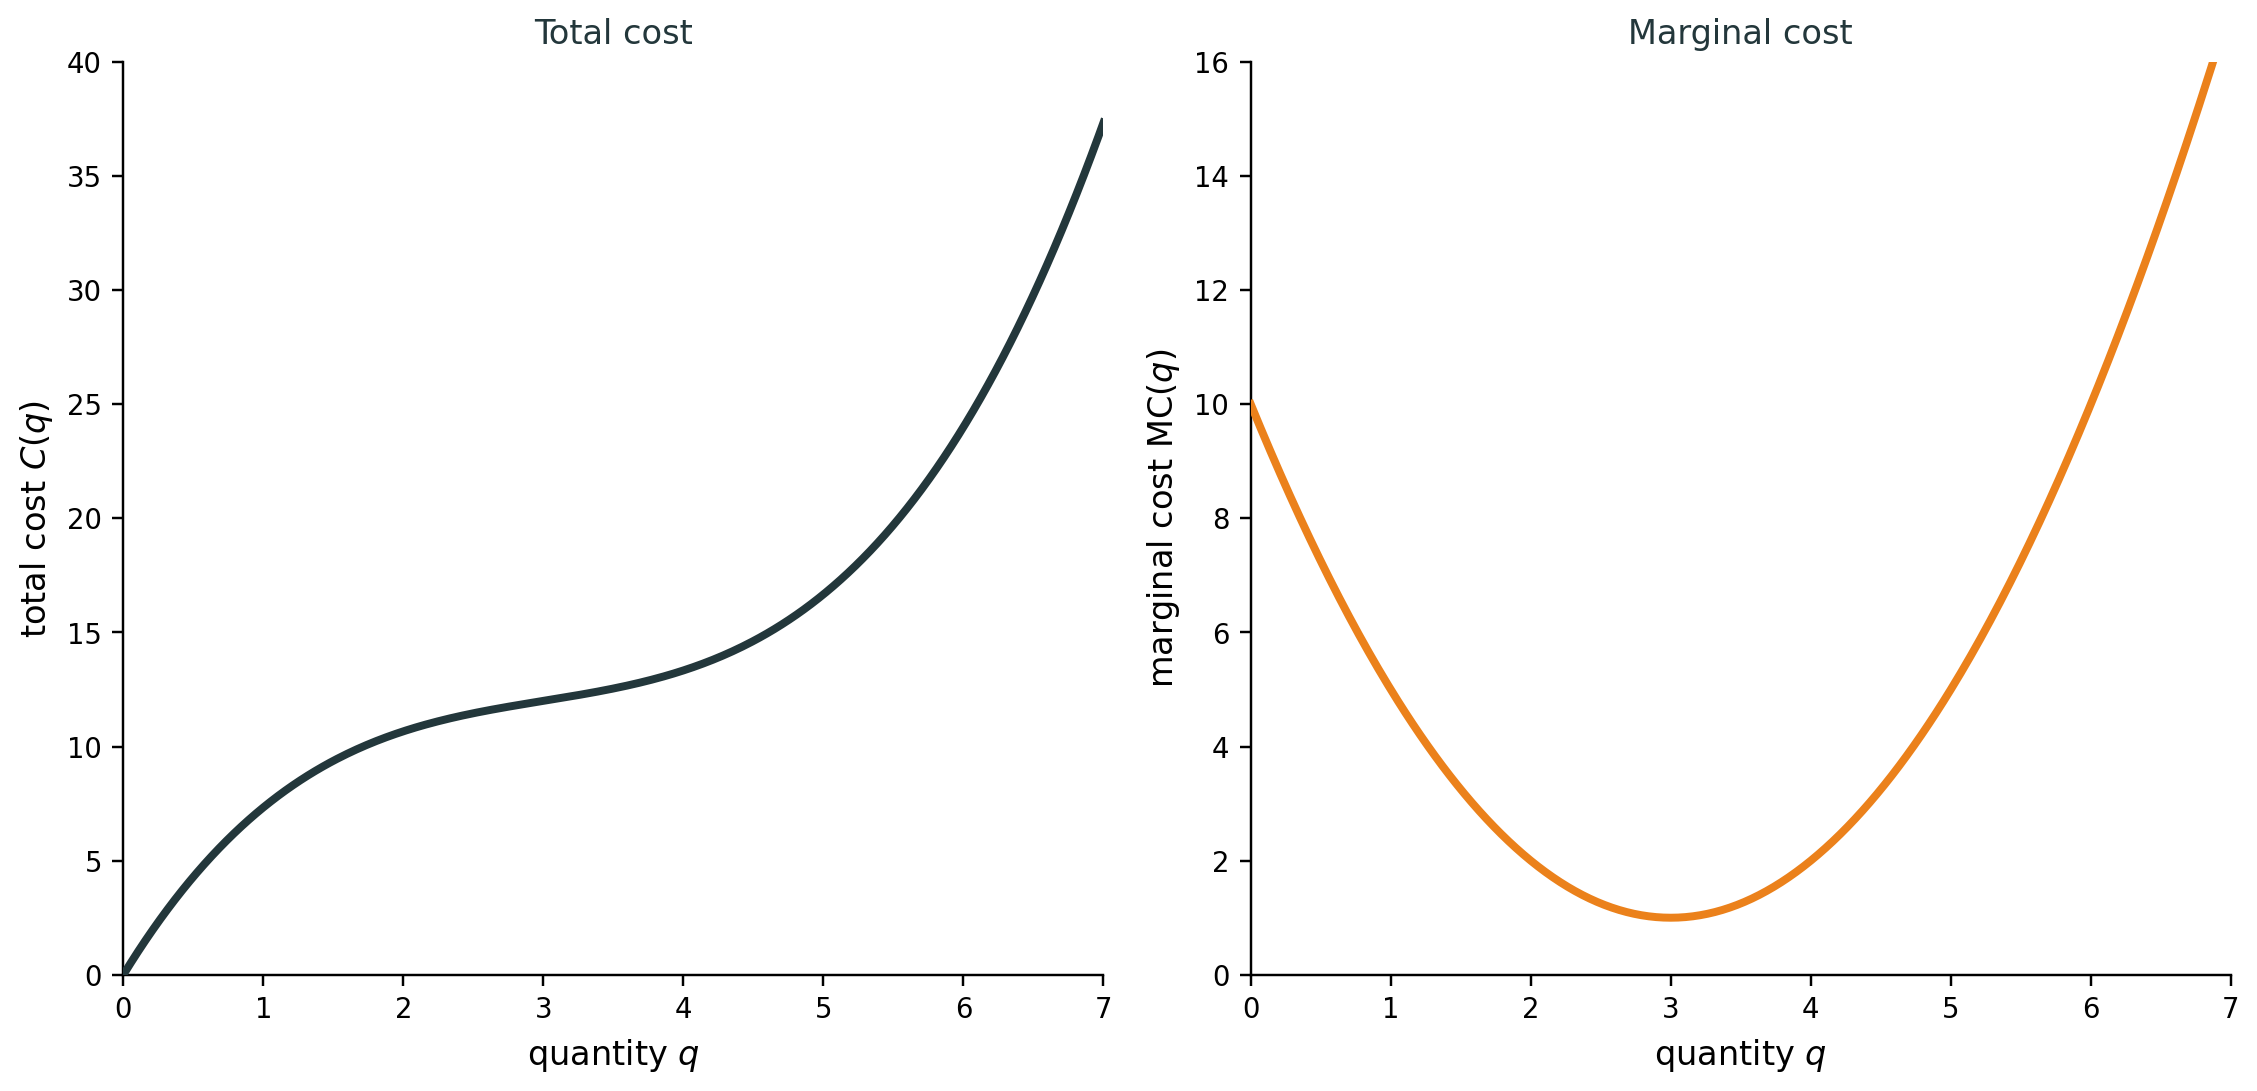
\includegraphics[width=0.96\textwidth,height=0.58\textheight,keepaspectratio]{figures/firm_cost.png}
  \end{center}
  
  Profit is $\pi(q)=5q-C(q)$. What quantity maximizes profit?
\end{frame}

\begin{frame}{4.1 The optimization problem}
  \small
  Consider: $\max_{x \in (a,b)} f(x)$ where $f$ is differentiable.
  
  \textbf{Goal:} Find conditions guaranteeing $x^*$ is a local maximum.
  
  Two types of conditions (always say \textbf{for what}):
  
  \begin{itemize}
    \item \textbf{Necessary for local max:} Must hold at any interior local max, but does not by itself guarantee a local max
    
    \item \textbf{Sufficient for local max:} If they hold, $x^*$ is definitely a local max (but need not be the only way to get one)
  \end{itemize}
\end{frame}

\begin{frame}{4.1 Necessary conditions at a local max}
  \small
  If $x^*$ is an interior local maximum, the graph looks like this:
  
  \begin{center}
    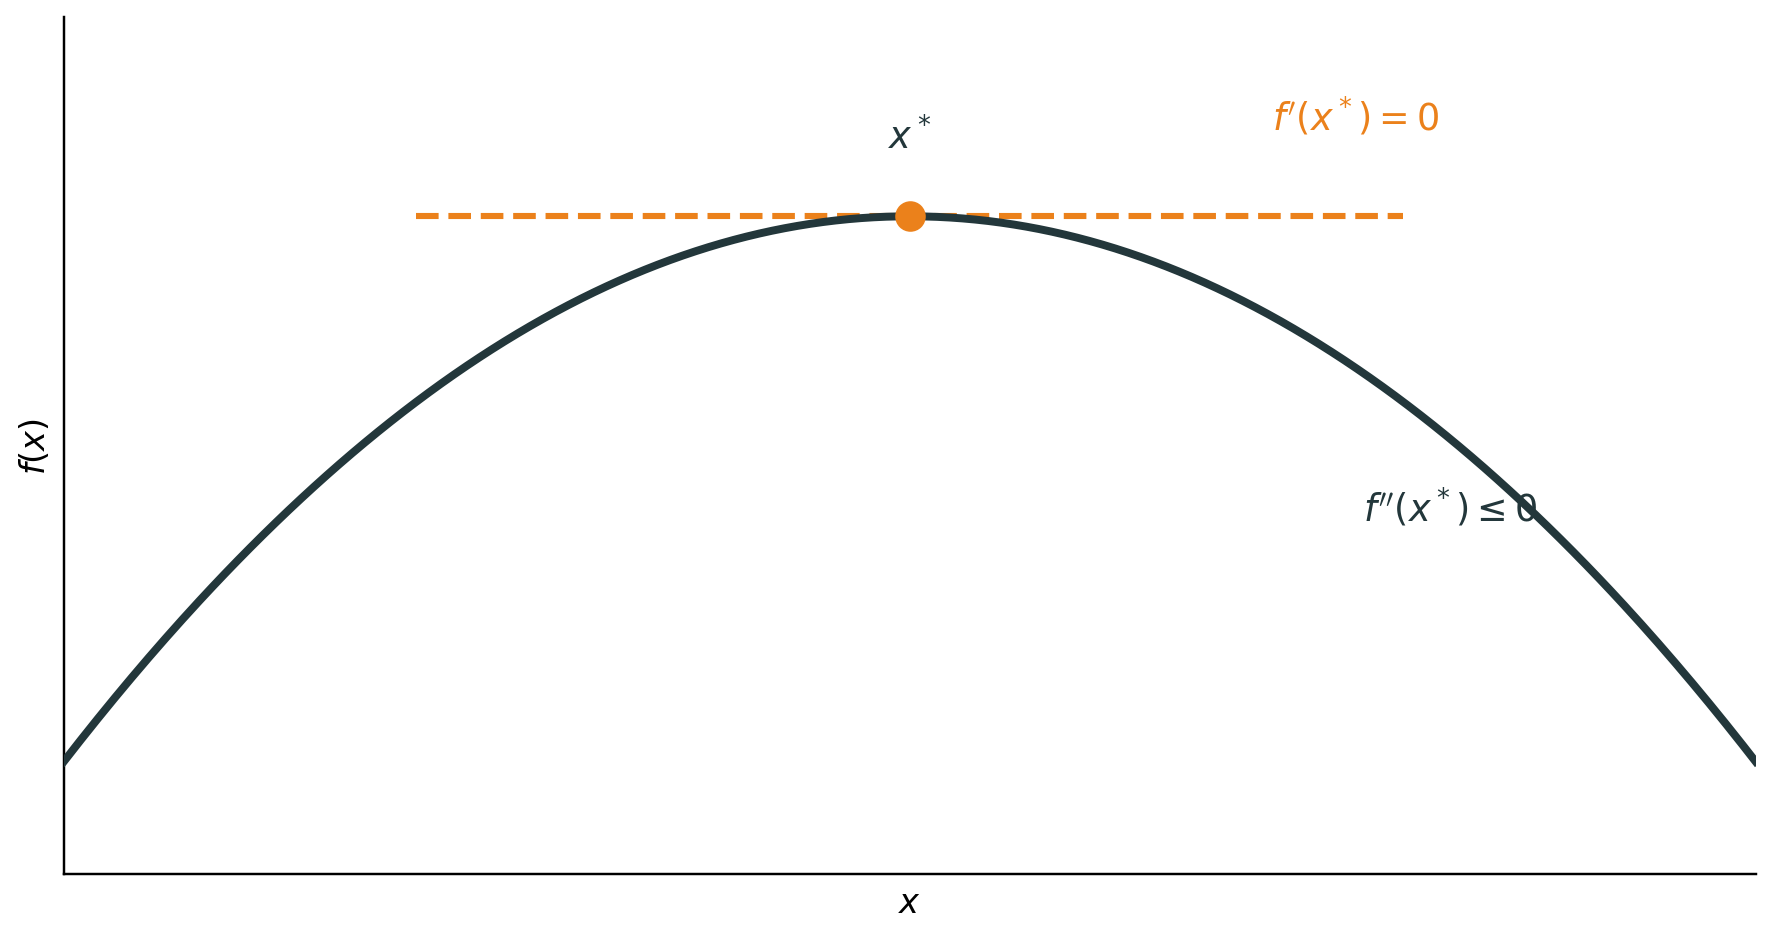
\includegraphics[width=0.82\textwidth,height=0.48\textheight,keepaspectratio]{figures/local_max_necessary.png}
  \end{center}
  
  The tangent is flat, so $f'(x^*)=0$. The curve bends down, so $f''(x^*)\leq 0$.
\end{frame}

\begin{frame}{4.1 Local conditions}
  \small
  At an interior critical point $x^*$ ($f'(x^*)=0$) with $f \in C^2$:
  
  \textbf{Necessary (1).} Local maximum $\Rightarrow$ $f'(x^*)=0$. \textbf{Not sufficient.}
  
  \textbf{Necessary (2).} Local maximum $\Rightarrow$ $f''(x^*)\leq 0$. \textbf{Not sufficient} (e.g.\ $x^3$ at $0$).
  
  \textbf{Sufficient.} If $f'(x^*)=0$ and $f''(x^*)<0$, then strict local maximum. \textbf{Not necessary} (e.g.\ $-x^4$ at $0$).
  
  \hfill\hyperlink{appendix:soc_1d}{\scriptsize Proofs: Appendix A.1 \InterestOnly}
\end{frame}

\begin{frame}{4.1 $f''\leq 0$ is not sufficient}
  \small
  $f(x)=x^3$ at $x^*=0$: $f'(0)=0$ and $f''(0)=0\leq 0$, but this is not a local maximum.
  
  \begin{center}
    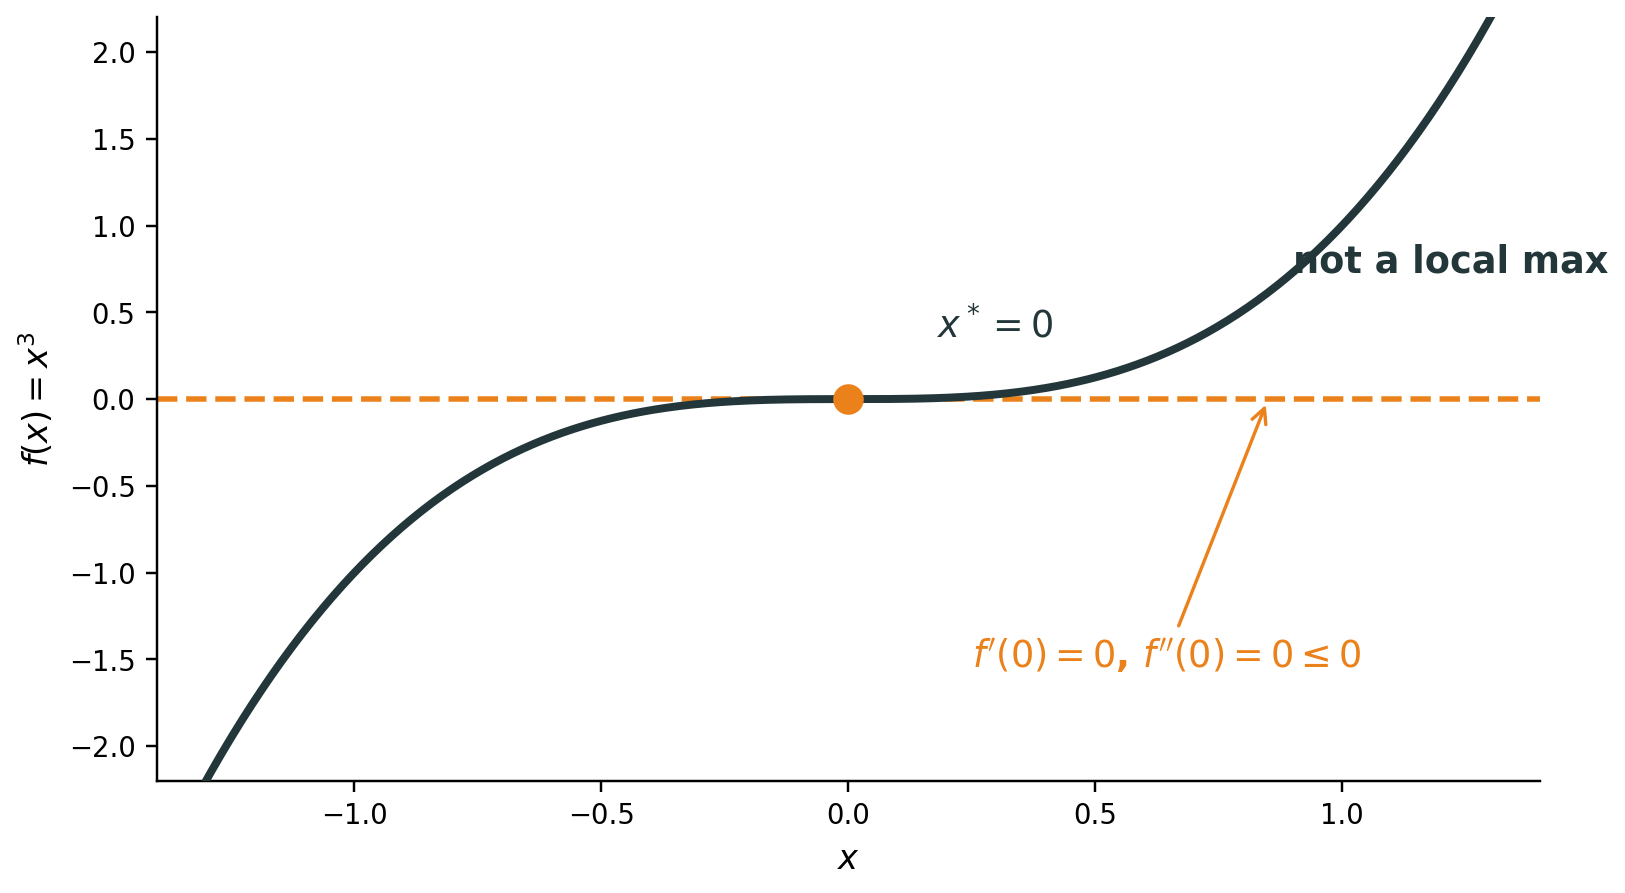
\includegraphics[width=0.82\textwidth,height=0.50\textheight,keepaspectratio]{figures/soc_not_sufficient.png}
  \end{center}
\end{frame}

\QFrame{4.1 Exercise: Finding critical points}
  \small
  \textbf{Exercise.} For the firm, $\pi(q)=5q-C(q)=-\tfrac13 q^3+3q^2-5q$ on $q\geq 0$. Find all critical points and classify each.
  
  \textbf{Solution.}
  
  \begin{itemize}
    \item $\pi'(q)=5-\mathrm{MC}(q)=-q^2+6q-5=-(q-1)(q-5)=0$ at $q=1,5$
    
    \item $\pi''(q)=-2q+6$, so $\pi''(1)=4>0$ --- \textbf{local minimum}
    
    \item $\pi''(5)=-4<0$ --- \textbf{local maximum} (sufficient SOC)
  \end{itemize}
  
  FOC gives two $p=\mathrm{MC}$ points; SOC keeps only the peak at $q=5$.
\end{frame}

\QFrame{4.1 Exercise: Why $p=\mathrm{MC}$}
  \small
  \textbf{Exercise.} Why must $p=\mathrm{MC}$ at an interior profit maximum?
  
  \begin{center}
    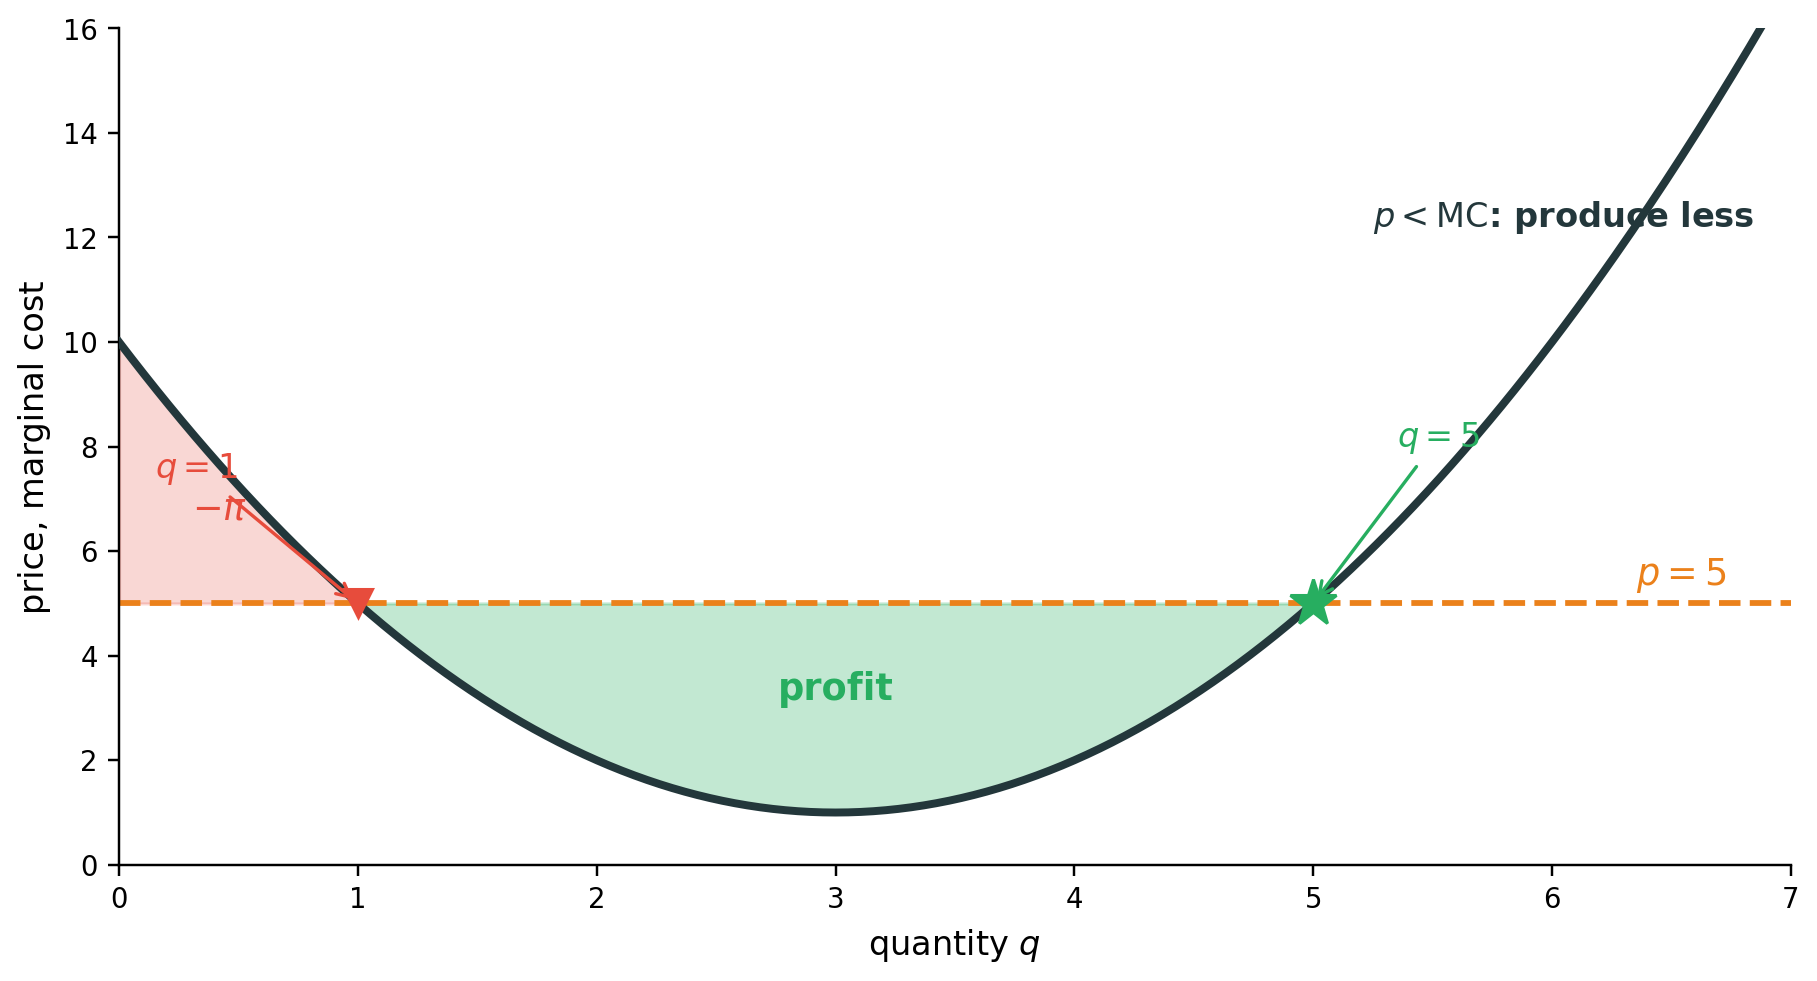
\includegraphics[width=0.78\textwidth,height=0.38\textheight,keepaspectratio]{figures/price_equals_mc.png}
  \end{center}
  
  \textbf{Solution.} One more unit earns $p$ and costs $\mathrm{MC}$. Profit is the signed area between $p$ and $\mathrm{MC}$: add area where $p>\mathrm{MC}$, subtract where $p<\mathrm{MC}$.
  
  Expand where $p>\mathrm{MC}$, cut where $p<\mathrm{MC}$, so $p=\mathrm{MC}$. SOC keeps the rising-MC point $q=5$.
\end{frame}

\begin{frame}{4.1 From local to global}
  \small
  A local maximum need not be a global maximum:
  
  \begin{center}
    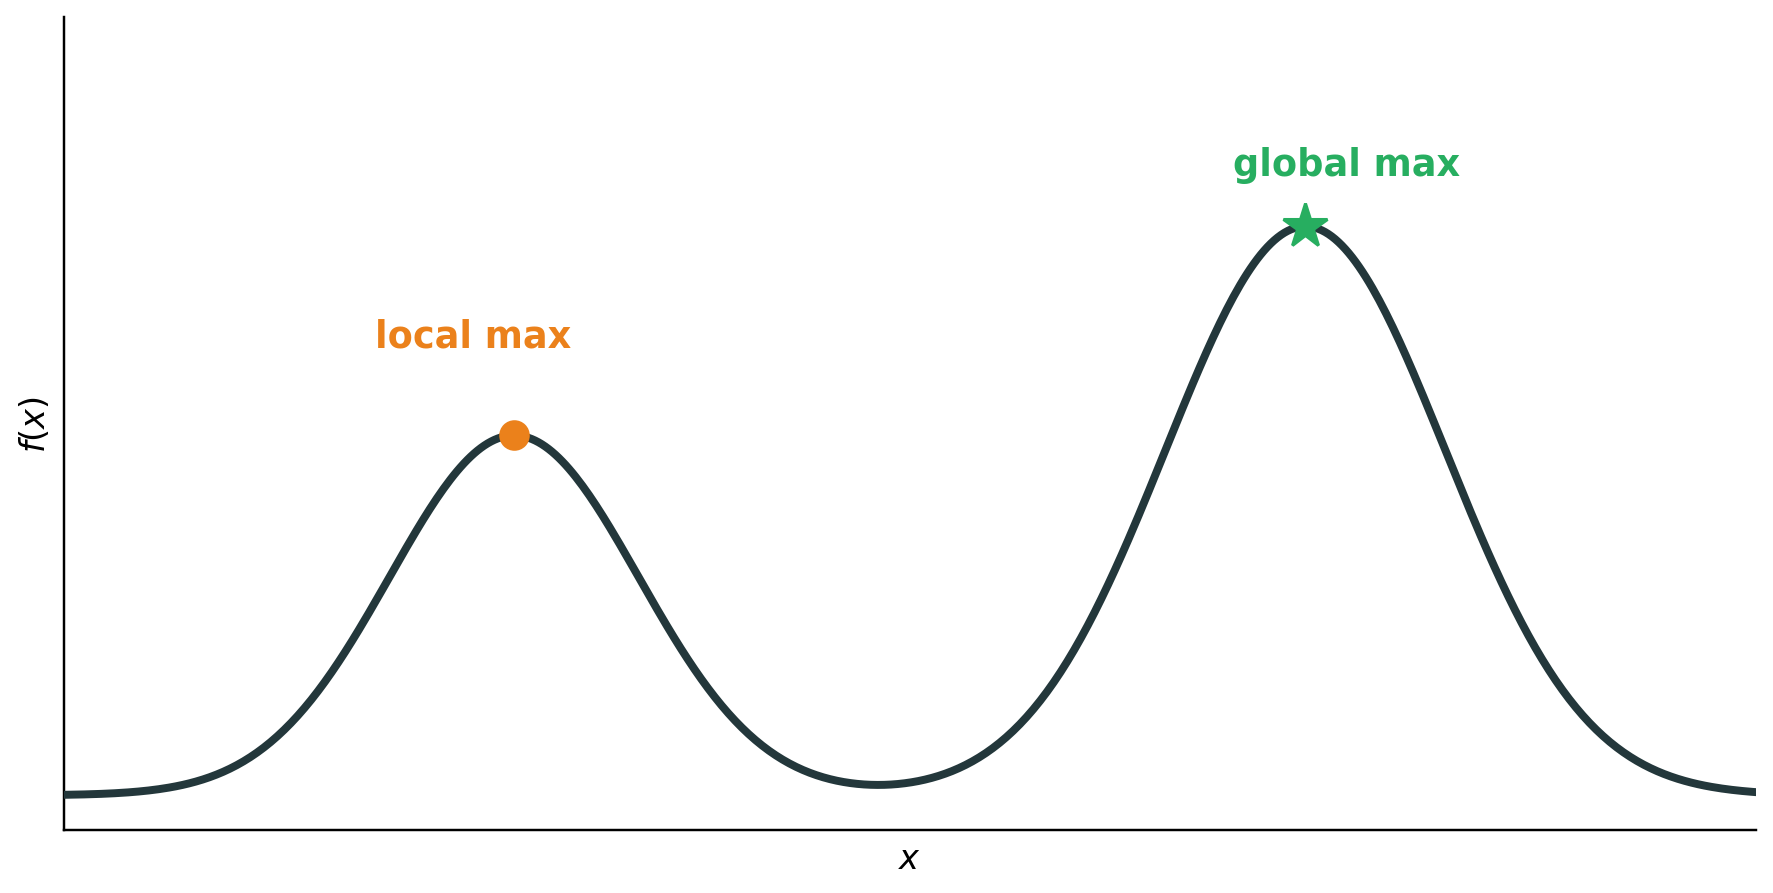
\includegraphics[width=0.82\textwidth,height=0.46\textheight,keepaspectratio]{figures/local_not_global.png}
  \end{center}
  
  \textbf{Question:} When does a critical point guarantee a \textbf{global} maximum?
  
  \textbf{Answer:} When $f$ is \textbf{concave}.
\end{frame}

%==============================================================================
\section{4.2 --- Concavity, Convexity, and Quasiconcavity}
%==============================================================================

\begin{frame}{4.2 (1) Chord definition}
  \small
  \textbf{(1) Concave.} For all $x, y$ and $\lambda \in [0,1]$:
  \[
    f(\lambda x + (1-\lambda)y) \geq \lambda f(x) + (1-\lambda)f(y).
  \]
  The graph lies \textbf{above} its chords (convex reverses the inequality).
  
  \begin{center}
    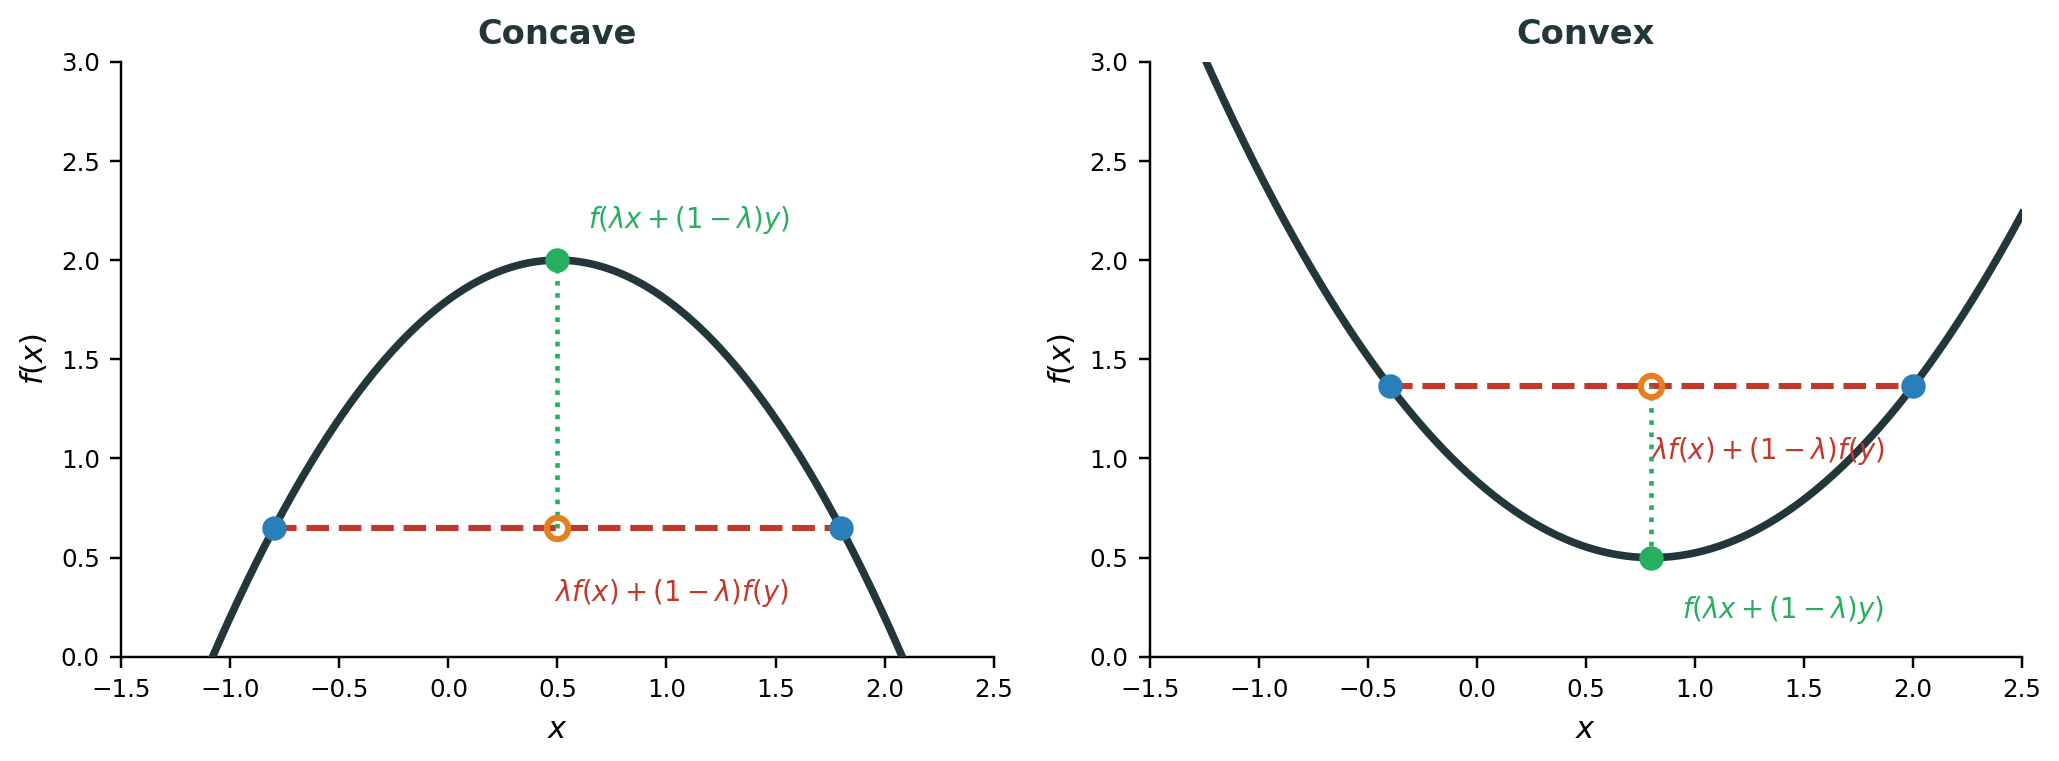
\includegraphics[width=0.92\textwidth,height=0.50\textheight,keepaspectratio]{figures/concave_chords.png}
  \end{center}
\end{frame}

\begin{frame}{4.2 (2) Tangent characterization}
  \small
  \textbf{(2) Concave (differentiable).} For all $x, y$:
  \[
    f(y) \leq f(x) + f'(x)(y-x).
  \]
  
  \textbf{Theorem.} For $f \in C^1$: $(1) \Leftrightarrow (2)$.
  
  \begin{center}
    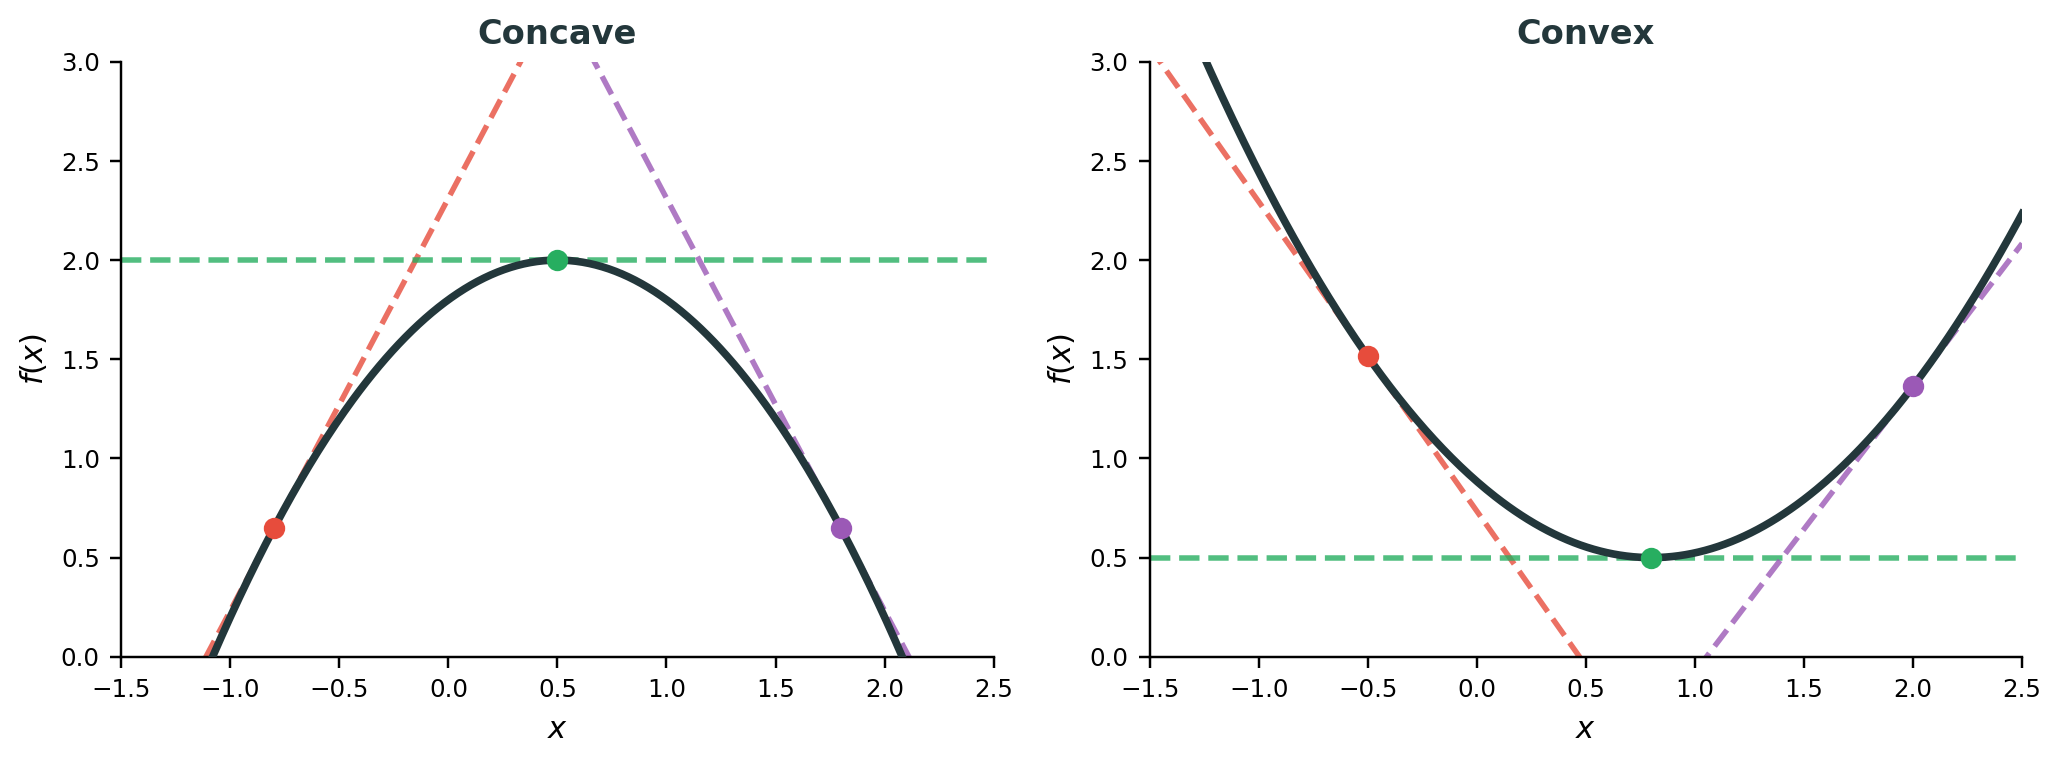
\includegraphics[width=0.92\textwidth,height=0.46\textheight,keepaspectratio]{figures/concave_tangents.png}
  \end{center}
  
  \hfill\hyperlink{appendix:concave_12}{\scriptsize Proof: Appendix A.2 \InterestOnly}
\end{frame}

\begin{frame}{4.2 (3) Second derivative condition}
  \small
  \textbf{(3) Concave ($C^2$).} $f''(x) \leq 0$ for all $x$ --- tangent slope $f'(x)$ is \textbf{decreasing}.
  
  \textbf{Theorem.} For $f \in C^2$: $(2) \Leftrightarrow (3)$.
  
  \begin{center}
    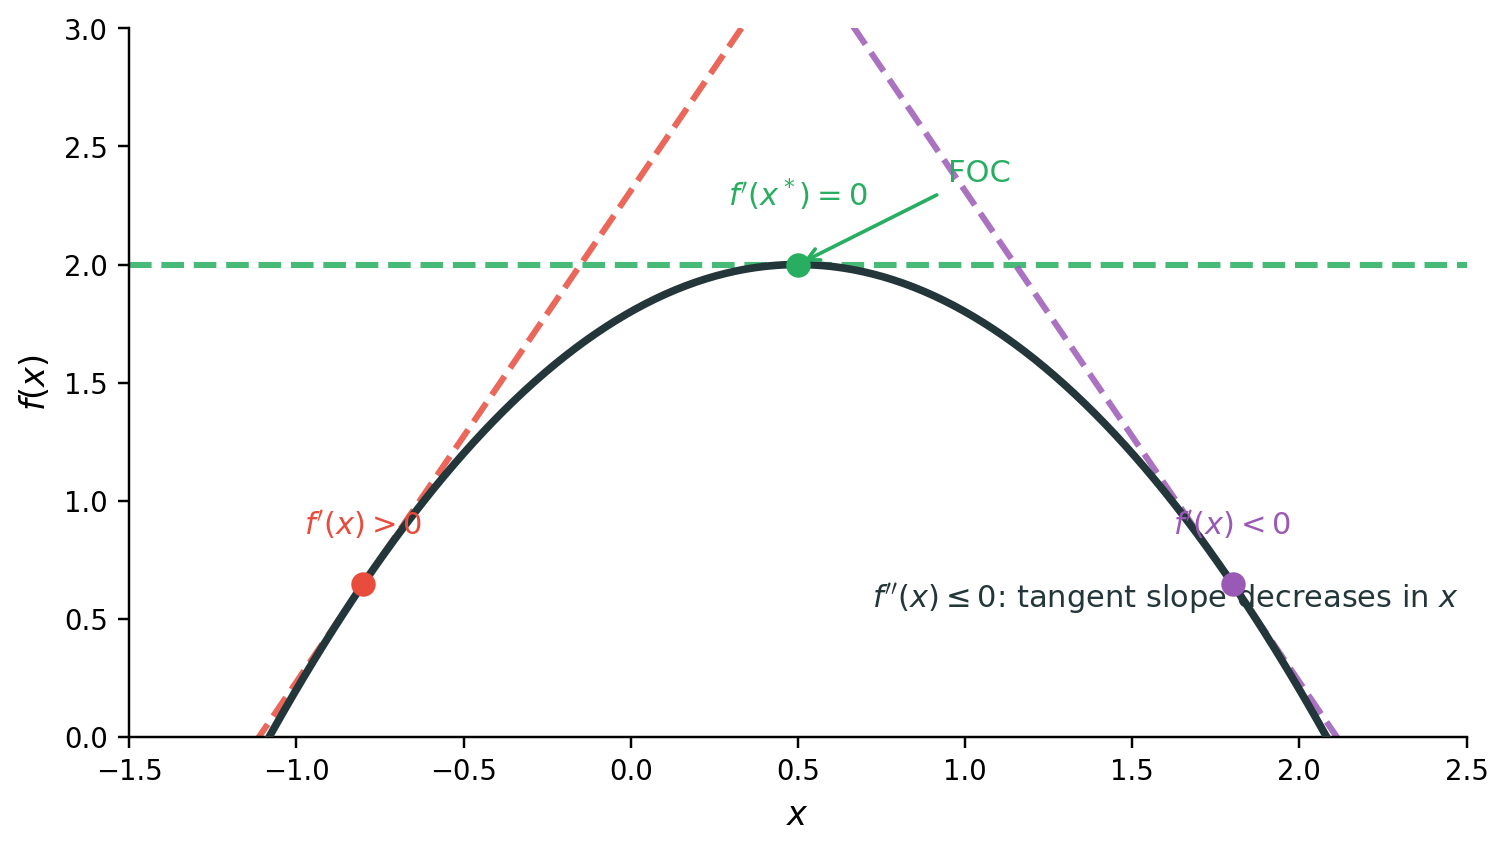
\includegraphics[width=0.88\textwidth,height=0.44\textheight,keepaspectratio]{figures/concave_second_derivative.png}
  \end{center}
  
  At a maximum, FOC gives $f'(x^*)=0$: the tangent is \textbf{horizontal}.
  
  \hfill\hyperlink{appendix:concave_23}{\scriptsize Proof: Appendix A.3 \InterestOnly}
\end{frame}

\QFrame{4.2 Exercise: Concavity implies global max}
  \small
  \textbf{Exercise.} Prove that if $f$ is concave and $f'(x^*) = 0$, then $x^*$ is a global maximum.
  
  \textbf{Solution.}
  
  \begin{itemize}
    \item By tangent characterization: $f(y) \leq f(x^*) + f'(x^*)(y-x^*)$ for all $y$
    
    \item Since $f'(x^*) = 0$: $f(y) \leq f(x^*)$ for all $y$
    
    \item Therefore $x^*$ is a global maximum
  \end{itemize}
  
  Concavity is \textbf{sufficient for global max} once FOC holds (FOC is only necessary for local max).
\end{frame}

\begin{frame}{4.2 Concavity: Global condition}
  \small
  \textbf{Optimization.} When $f$ is concave, every local maximum is a global maximum. In particular, if $x^*$ satisfies $f'(x^*)=0$, then $x^*$ is a global maximum: $f(y) \leq f(x^*)$ for all $y$.
  
  \textbf{Three equivalent forms} ($f \in C^2$):
  \begin{enumerate}
    \item \textbf{Chords:} $f(\lambda x + (1-\lambda)y) \geq \lambda f(x) + (1-\lambda)f(y)$
    
    \item \textbf{Tangents:} $f(y) \leq f(x) + f'(x)(y-x)$
    
    \item \textbf{Second derivative:} $f''(x) \leq 0$
  \end{enumerate}
  
  \textbf{Geometry.} Graph above chords, below tangents; Taylor \textbf{overestimates} $f$.
\end{frame}

\begin{frame}{4.2 Convex functions: Global minimum}
  \small
  \textbf{Optimization.} When $f$ is convex, every local minimum is a global minimum. In particular, if $x^*$ satisfies $f'(x^*)=0$, then $x^*$ is a global minimum: $f(y) \geq f(x^*)$ for all $y$.
  
  \textbf{Three equivalent forms} ($f \in C^2$):
  \begin{enumerate}
    \item \textbf{Chords:} $f(\lambda x + (1-\lambda)y) \leq \lambda f(x) + (1-\lambda)f(y)$
    
    \item \textbf{Tangents:} $f(y) \geq f(x) + f'(x)(y-x)$
    
    \item \textbf{Second derivative:} $f''(x) \geq 0$
  \end{enumerate}
  
  \textbf{Geometry.} Graph below chords, above tangents; Taylor \textbf{underestimates} $f$.
\end{frame}

\begin{frame}{4.2 Strict concavity}
  \small
  \textbf{Optimization.} When $f$ is strictly concave, there is at most one global maximum. If $f'(x^*)=0$, then $x^*$ is the unique global maximum.
  
  \textbf{Three characterizations} ($f \in C^2$):
  \begin{enumerate}
    \item \textbf{Strict chords:} for $x \neq y$, $\lambda \in (0,1)$: $f(\lambda x+(1-\lambda)y) > \lambda f(x)+(1-\lambda)f(y)$
    
    \item \textbf{Strict tangents:} for $x \neq y$: $f(y) < f(x)+f'(x)(y-x)$
    
    \item \textbf{Second derivative:} $f''(x) < 0$ for all $x$ --- \textbf{sufficient but not necessary}
  \end{enumerate}
  
  \textbf{Example.} $f(x)=-x^4$: strictly concave, but $f''(0)=0$.
\end{frame}

\QFrame{4.2 Exercise: FOC, SOC, and global maximum}
  \small
  \textbf{Exercise.} For $f(x) = \ln(x) - x$ on $x > 0$, find critical points, verify SOC, and determine whether $x^*$ is a global maximum.
  
  \begin{columns}[T]
    \begin{column}{0.54\textwidth}
      \begin{center}
        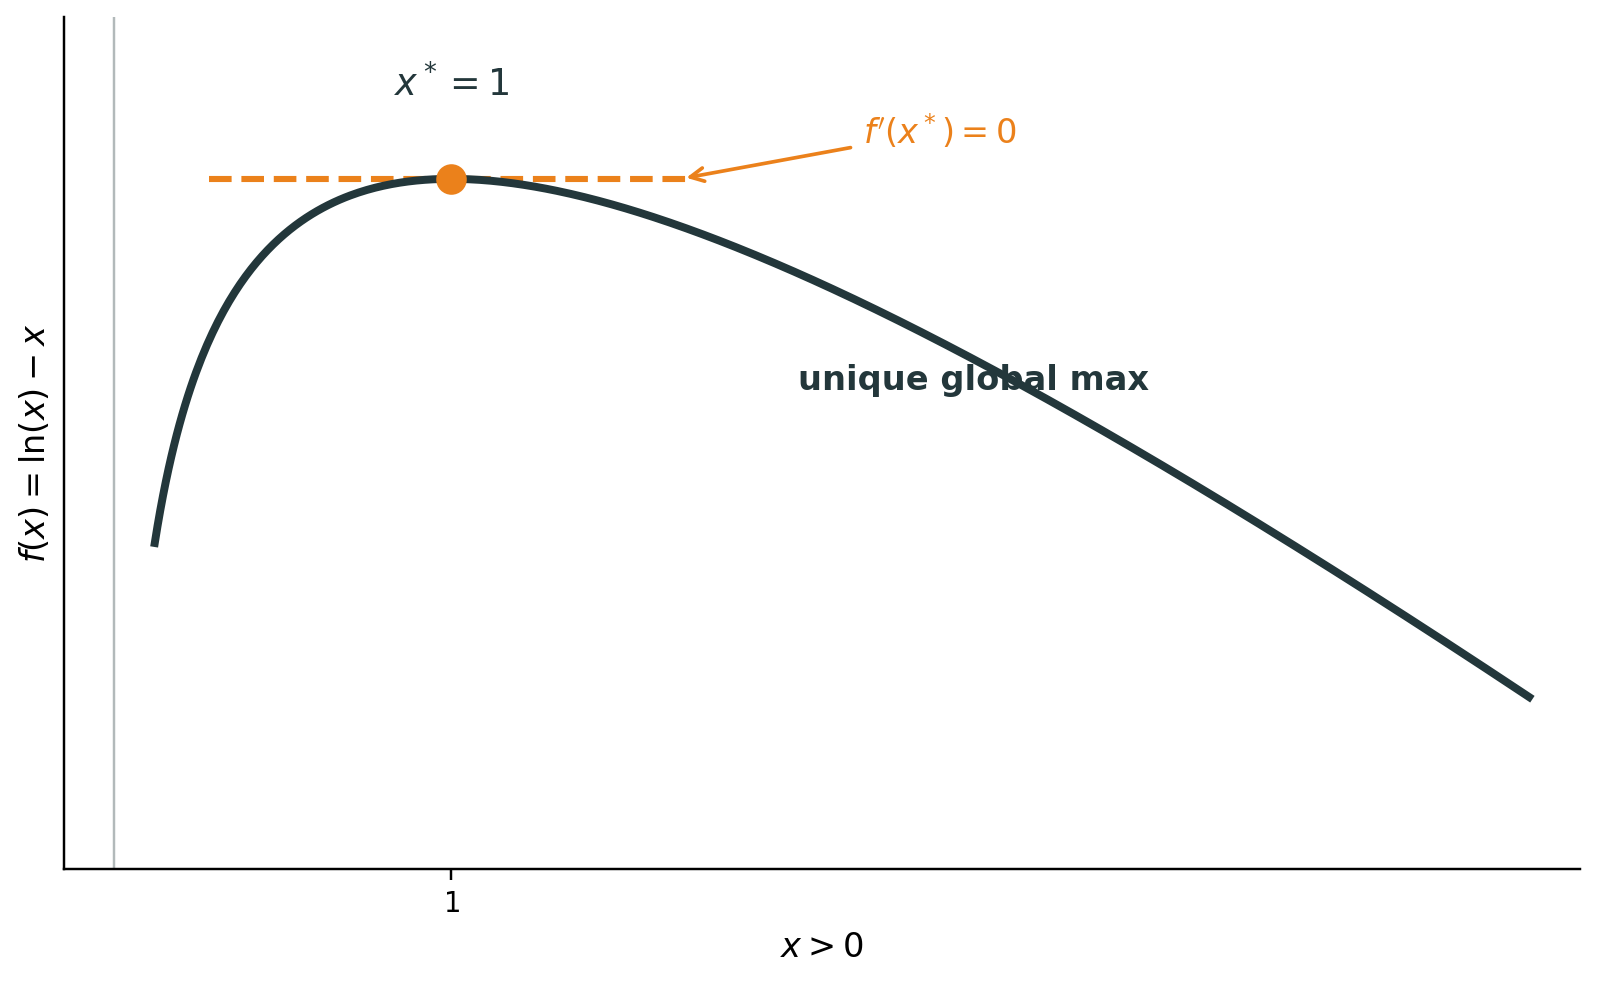
\includegraphics[width=\textwidth,height=0.58\textheight,keepaspectratio]{figures/ln_minus_x.png}
      \end{center}
    \end{column}
    \begin{column}{0.44\textwidth}
      \textbf{Solution.}
      \begin{itemize}
        \item $f'(x)=\frac{1}{x}-1=0$ gives $x^*=1$
        
        \item $f''(1)=-1<0$ $\Rightarrow$ strict local maximum
        
        \item $f''(x)=-\frac{1}{x^2}<0$ for all $x>0$, so $f$ is strictly concave
        
        \item Therefore $x^*=1$ is the unique \textbf{global} maximum
      \end{itemize}
    \end{column}
  \end{columns}
\end{frame}

\QFrame{4.2 Exercise: Testing concavity vs. convexity}
  \small
  \textbf{Exercise.} Determine if these functions are concave, convex, or neither:
  
  \textbf{(a)} $f(x) = -x^2$ on $\mathbb{R}$
  
  \begin{itemize}
    \item $f''(x) = -2 < 0$ for all $x$ $\Rightarrow$ \textbf{strictly concave}
  \end{itemize}
  
  \textbf{(b)} $f(x) = e^x$ on $\mathbb{R}$
  
  \begin{itemize}
    \item $f''(x) = e^x > 0$ for all $x$ $\Rightarrow$ \textbf{strictly convex}
  \end{itemize}
  
  \textbf{(c)} $f(x) = x^3$ on $\mathbb{R}$
  
  \begin{itemize}
    \item $f''(x) = 6x$ changes sign at $x = 0$ $\Rightarrow$ \textbf{neither} concave nor convex on all of $\mathbb{R}$
  \end{itemize}
\end{frame}

\begin{frame}{4.2 Example: Profit maximization}
  \small
  \textbf{Example.} Profit $\pi(q)=pq-C(q)$.
  
  \begin{itemize}
    \item \textbf{Decreasing returns:} marginal cost rises as output increases (e.g.\ $C(q)=q^2$)
    
    \item Then $\pi''(q)=-C''(q)<0$, so $\pi$ is concave
    
    \item FOC $\pi'(q^*)=0$ gives the \textbf{global} profit maximum, not just a local one
  \end{itemize}
\end{frame}

\begin{frame}{4.2 Local condition (multivariate)}
  \small
  At an interior critical point $\mathbf{x}^*$ ($\nabla f(\mathbf{x}^*)=\mathbf{0}$) with $f \in C^2$:
  
  \textbf{Necessary (1).} Local maximum $\Rightarrow$ $\nabla f(\mathbf{x}^*)=\mathbf{0}$. \textbf{Not sufficient.}
  
  \textbf{Necessary (2).} Local maximum $\Rightarrow$ $H_f(\mathbf{x}^*)$ negative semidefinite. \textbf{Not sufficient} (e.g.\ $x^3$ at $(0,0)$).
  
  \textbf{Sufficient.} If $\nabla f(\mathbf{x}^*)=\mathbf{0}$ and $H_f(\mathbf{x}^*)$ negative definite, then strict local maximum. \textbf{Not necessary} (e.g.\ $-(x^4+y^4)$ at $(0,0)$).
  
  Same pattern as 1D: $f''(x^*)\leq 0$ necessary; $f''(x^*)<0$ sufficient but not necessary.
  
  \hfill\hyperlink{appendix:multivariate_soc}{\scriptsize Proofs: Appendix A.5 \InterestOnly}
\end{frame}

\begin{frame}{4.2 Global condition (multivariate)}
  \small
  \textbf{Optimization.} When $f$ is concave, every local maximum is a global maximum. In particular, if $\nabla f(\mathbf{x}^*)=\mathbf{0}$, then $\mathbf{x}^*$ is a global maximum: $f(\mathbf{y}) \leq f(\mathbf{x}^*)$ for all $\mathbf{y}$.
  
  \textbf{Three equivalent forms} ($f \in C^2$):
  \begin{enumerate}
    \item \textbf{Chords:} $f(\lambda \mathbf{x}+(1-\lambda)\mathbf{y}) \geq \lambda f(\mathbf{x})+(1-\lambda)f(\mathbf{y})$
    
    \item \textbf{Tangents:} $f(\mathbf{y}) \leq f(\mathbf{x})+\nabla f(\mathbf{x})^\top(\mathbf{y}-\mathbf{x})$
    
    \item \textbf{Hessian:} $H_f(\mathbf{x})$ is NSD for all $\mathbf{x}$ (recall, Day~3)
  \end{enumerate}
  
  \textbf{Geometry.} For $f(x,y)$, the surface $z=f(x,y)$ lies \textbf{below} its tangent plane; shape is an inverted bowl.
  
  \hfill\hyperlink{appendix:concave_12}{\scriptsize $(1)\Leftrightarrow(2)$: A.2 \InterestOnly}\quad
  \hyperlink{appendix:multivariate_concave}{\scriptsize $(2)\Leftrightarrow(3)$: A.4 \InterestOnly}
\end{frame}

\begin{frame}{4.2 Negative semidefinite}
  \small
  \textbf{Recall (end of Day~3).} For symmetric $H \in \mathbb{R}^{n \times n}$, the following are equivalent (proved on Day~3):
  
  \begin{itemize}
    \item \textbf{Quadratic form:} $\mathbf{v}^\top H \mathbf{v} \leq 0$ for all $\mathbf{v} \in \mathbb{R}^n$
    
    \item \textbf{Eigenvalues:} every $\lambda_i \leq 0$
    
    \item \textbf{Diagonal entries:} $H_{ii} \leq 0$ for all $i$ (necessary); if $H$ is diagonal, NSD $\Leftrightarrow$ all $H_{ii} \leq 0$
    
    \item \textbf{Leading principal minors:} $(-1)^k \Delta_k \geq 0$ for $k=1,\ldots,n$
  \end{itemize}
  
  \textbf{$n=2$.} $H = \begin{bmatrix} a & b \\ b & c \end{bmatrix}$ is NSD iff $a \leq 0$, $c \leq 0$, and $ac - b^2 \geq 0$.
\end{frame}

\begin{frame}{4.2 Multivariate concavity: Geometry}
  \small
  For $f(x,y)$, the graph $z=f(x,y)$ is a \textbf{surface in 3D}.
  
  \begin{center}
    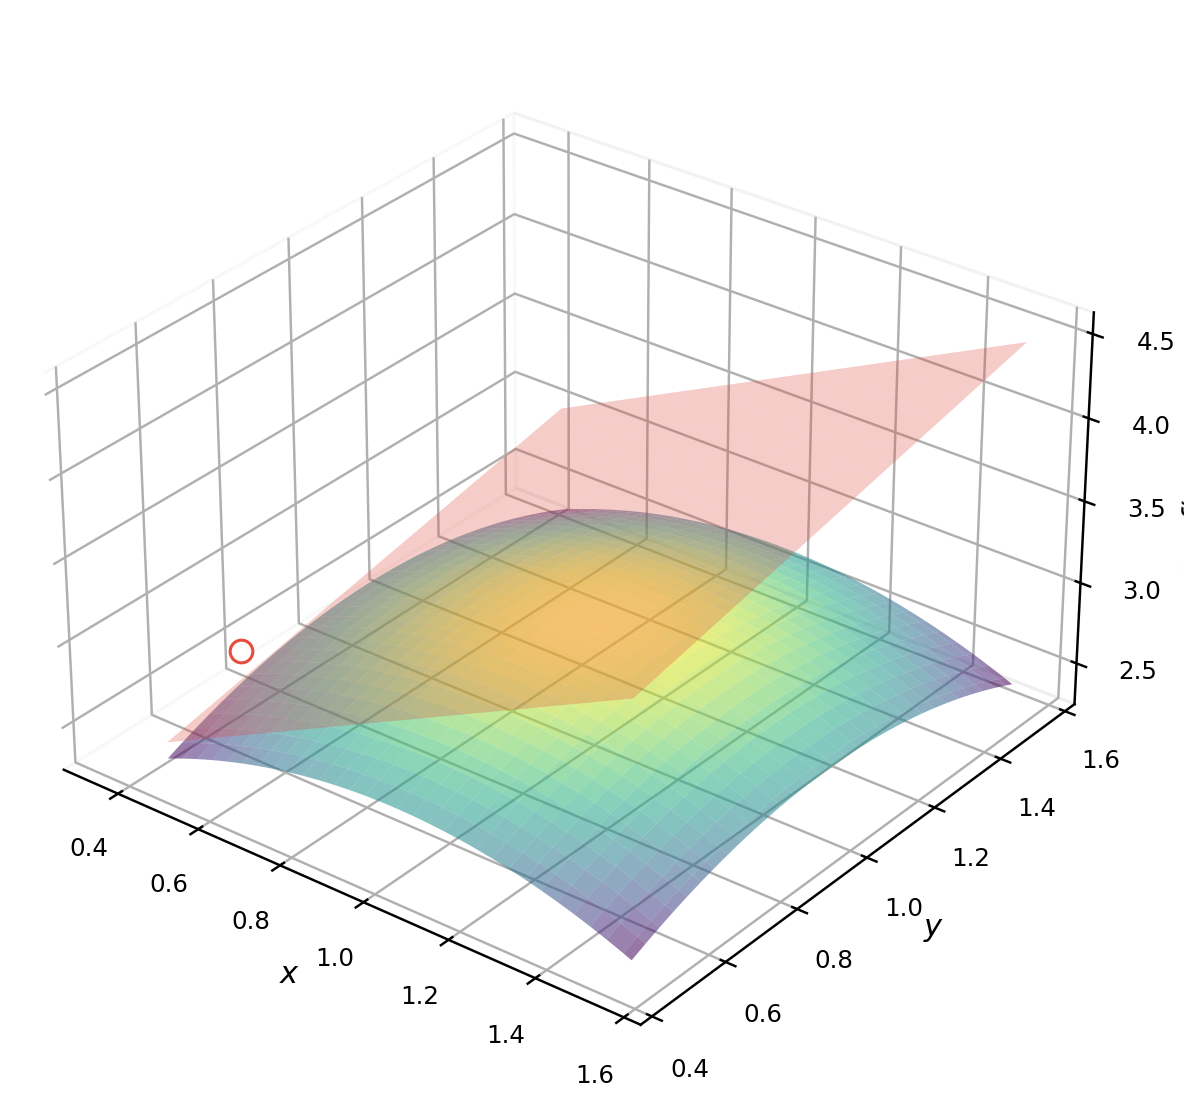
\includegraphics[width=0.58\textwidth,height=0.52\textheight,keepaspectratio]{figures/concave_tangent_plane_3d.png}
  \end{center}
  
  Concavity: surface lies \textbf{below} its tangent plane; shape is an inverted bowl.
\end{frame}

\begin{frame}{4.2 One-dimensional quasiconcave function}
  \small
  Concavity gives a unique peak, but it is \textbf{too strong}: a single-peaked $f$ can fail the chord test.
  
  \begin{center}
    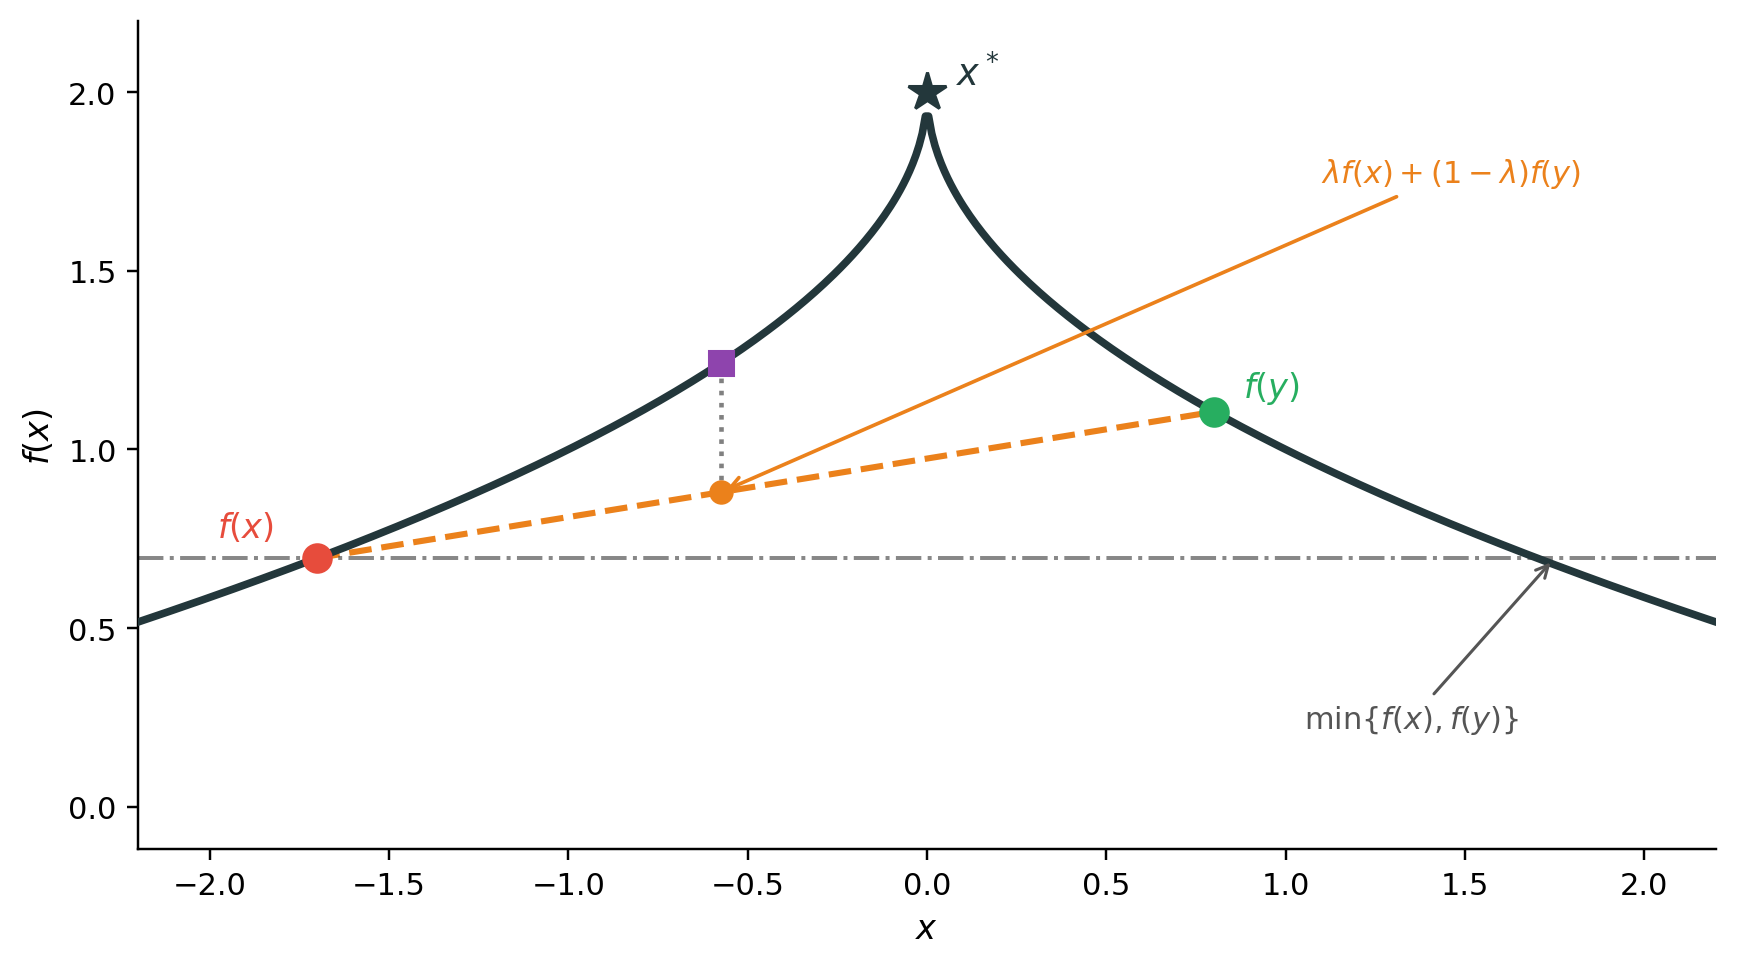
\includegraphics[width=0.92\textwidth,height=0.52\textheight,keepaspectratio]{figures/quasiconcave_1d.png}
  \end{center}
  
  The graph can lie \textbf{below} the chord (not concave) and still stay above $\min\{f(x),f(y)\}$ --- one peak, still good for maximization.
\end{frame}

\begin{frame}{4.2 Quasiconcave functions: Two definitions}
  \small
  \textbf{Definition A (segment).} $f$ is \textbf{quasiconcave} if for all $x, y$ and $\lambda \in [0,1]$:
  
  \[
    f(\lambda x + (1-\lambda)y) \geq \min\{f(x), f(y)\}.
  \]
  
  Along any segment, $f$ stays at least as high as the lower endpoint.
  
  \textbf{Definition B (upper contours).} $f$ is quasiconcave if upper contour sets $S_t = \{\mathbf{x}: f(\mathbf{x}) \geq t\}$ are convex for all $t$.
\end{frame}

\begin{frame}{4.2 Two-dimensional upper contour sets}
  \begin{center}
    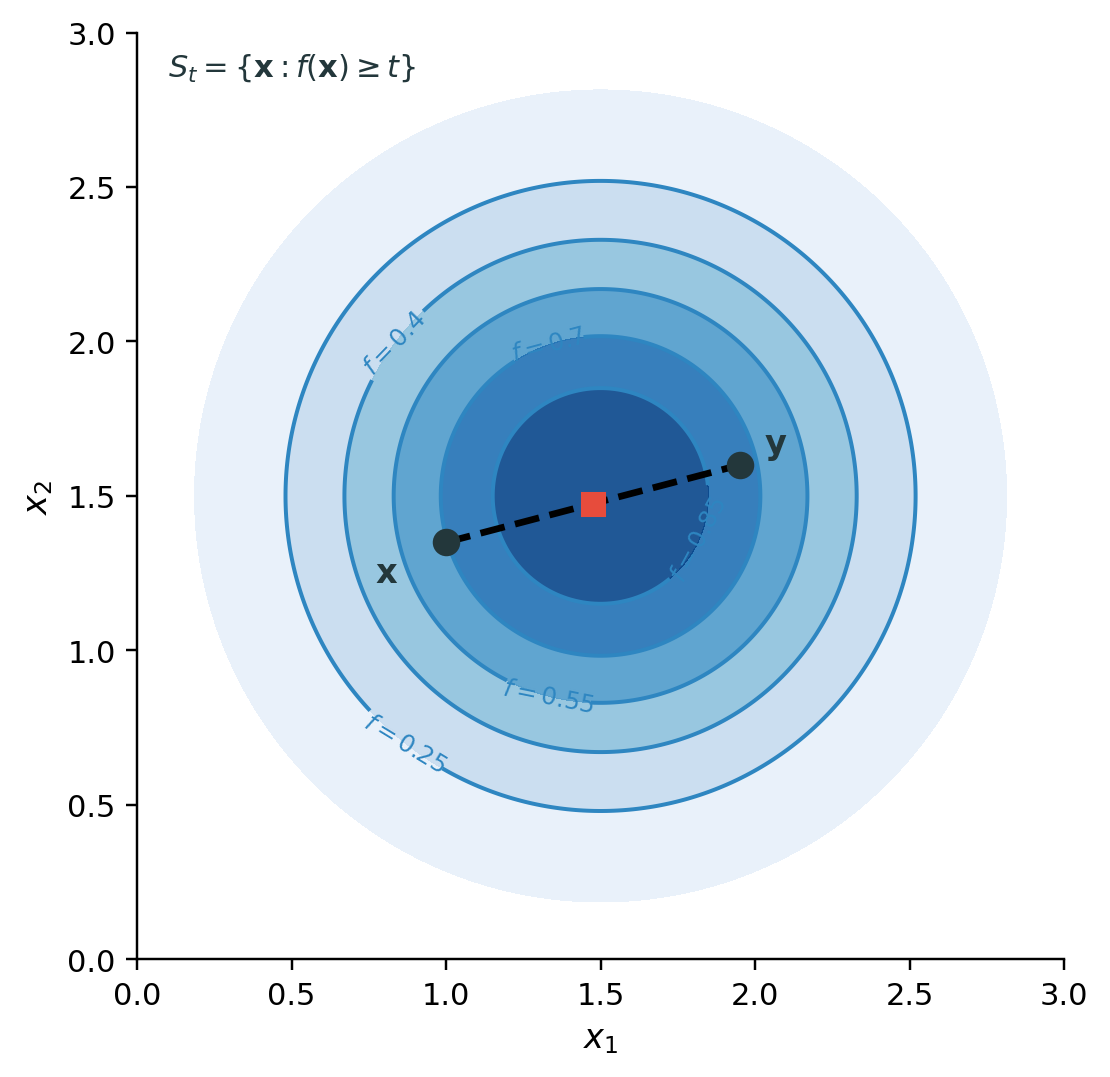
\includegraphics[height=0.74\textheight]{figures/quasiconcave_intuition.png}
  \end{center}
\end{frame}

\begin{frame}{4.2 Equivalence: segment vs. upper contours}
  \small
  \textbf{Theorem.} Definitions A and B are equivalent.

  \textbf{A:} $f(\lambda x+(1-\lambda)y)\geq \min\{f(x),f(y)\}$.
  
  \textbf{B:} $S_t=\{\mathbf{x}: f(\mathbf{x})\geq t\}$ is convex for every $t$.
  
  \textbf{Proof (A $\Rightarrow$ B).} Let $\mathbf{x}, \mathbf{y} \in S_t$.
  
  \begin{itemize}
    \item Then $f(\mathbf{x}) \geq t$, $f(\mathbf{y}) \geq t$
    
    \item For $\lambda \in [0,1]$: $f(\lambda\mathbf{x}+(1-\lambda)\mathbf{y}) \geq \min\{f(\mathbf{x}),f(\mathbf{y})\} \geq t$
    
    \item The segment stays in $S_t$, so $S_t$ is convex
  \end{itemize}
  
  \textbf{Proof (B $\Rightarrow$ A).} WLOG $f(\mathbf{x}) \geq f(\mathbf{y})$.
  
  \begin{itemize}
    \item Then $\mathbf{x}, \mathbf{y} \in S_{f(\mathbf{y})}$
    
    \item By convexity of $S_{f(\mathbf{y})}$: the segment is in $S_{f(\mathbf{y})}$
    
    \item So $f(\text{segment}) \geq f(\mathbf{y}) = \min\{f(\mathbf{x}),f(\mathbf{y})\}$
  \end{itemize}
\end{frame}

\begin{frame}{4.2 Quasiconcavity and monotone transforms}
  \small
  \textbf{Theorem.} If $f$ is quasiconcave and $\varphi:\mathbb{R}\to\mathbb{R}$ is \textbf{strictly increasing}, then $g=\varphi\circ f$ is quasiconcave.
  
  \textbf{Proof (upper contours).} For any $t$, since $\varphi$ is increasing, $\varphi^{-1}$ exists and
  \[
    \{\mathbf{x}: g(\mathbf{x}) \geq t\}
    =
    \{\mathbf{x}: f(\mathbf{x}) \geq \varphi^{-1}(t)\},
  \]
  which is convex because $f$ is quasiconcave.
  
  \textbf{Example.} Quasiconcave utility $u$ stays quasiconcave under $\ln u$, $u^{1/2}$, etc. --- same indifference curves, same optimization.
\end{frame}

\begin{frame}{4.2 Concave implies quasiconcave}
  \small
  \textbf{Theorem.} Concave $\Rightarrow$ quasiconcave, but not conversely.
  
  \textbf{Proof.} For concave $f$ and any $x, y$, $\lambda \in [0,1]$:
  
  \begin{itemize}
    \item By concavity: $f(\lambda x + (1-\lambda)y) \geq \lambda f(x) + (1-\lambda)f(y)$
    
    \item WLOG $f(x) \geq f(y)$, so $\min\{f(x),f(y)\} = f(y)$
    
    \item Then: $\lambda f(x) + (1-\lambda)f(y) \geq f(y) = \min\{f(x),f(y)\}$
    
    \item Therefore: $f(\lambda x + (1-\lambda)y) \geq \min\{f(x),f(y)\}$
  \end{itemize}
  
  This is the definition of quasiconcavity. The converse fails: e.g., sigmoid is quasiconcave but not concave.
\end{frame}

\begin{frame}{4.2 Quasiconvex functions}
  \small
  \textbf{Definition.} $f$ is \textbf{quasiconvex} if for all $x, y$ and $\lambda \in [0,1]$:
  
  \[
    f(\lambda x + (1-\lambda)y) \leq \max\{f(x), f(y)\}.
  \]
  
  Equivalently: lower contour sets $\{\mathbf{x}: f(\mathbf{x}) \leq t\}$ are convex.
  
  \textbf{Key relationship:} $f$ quasiconcave $\Leftrightarrow$ $-f$ quasiconvex.
  
  \textbf{Example:} $f(x) = x^2$ is quasiconvex (lower sets $[-a, a]$ are convex).
\end{frame}

\begin{frame}{4.2 Log-concave and hierarchy}
  \small
  \textbf{Definition.} $f$ is \textbf{log-concave} if $\ln f$ is concave (for $f > 0$).
  
  \textbf{Hierarchy (strongest to weakest):}
  
  \begin{enumerate}
    \item Concave
    
    \item Log-concave
    
    \item Quasiconcave
  \end{enumerate}
  
  \textbf{Relationships:}
  
  \begin{itemize}
    \item Concave and positive $\Rightarrow$ log-concave
    
    \item Log-concave $\Rightarrow$ quasiconcave
  \end{itemize}
  
  \hfill\hyperlink{appendix:logconcave}{\scriptsize See Appendix A.6 for proofs \InterestOnly}
\end{frame}

\begin{frame}{4.2 Economic examples}
  \small
  \textbf{Cobb--Douglas:} $u(x_1, x_2) = x_1^\alpha x_2^{1-\alpha}$
  
  \begin{itemize}
    \item \textbf{Not concave} for $\alpha \in (0,1)$: the Hessian is not NSD everywhere
    
    \item \textbf{Log-concave} and \textbf{quasiconcave} for all $\alpha \in (0,1)$
  \end{itemize}
  
  \textbf{CES:} $u = (x_1^\rho + x_2^\rho)^{1/\rho}$
  
  \begin{itemize}
    \item Log-concave for certain parameter ranges
    
    \item Quasiconcave more generally
  \end{itemize}
  
  \textbf{Why this matters:} FOC gives global max on convex budget set.
\end{frame}

\QFrame{4.2 Exercise: Cobb--Douglas quasiconcavity}
  \small
  \textbf{Exercise.} Show $u(x_1, x_2) = x_1^\alpha x_2^{1-\alpha}$ is quasiconcave on $\mathbb{R}^2_{++}$.
  
  \textbf{Solution.} Definition B: show $S_t = \{\mathbf{x} \in \mathbb{R}^2_{++} : u(\mathbf{x}) \geq t\}$ is convex for every $t$.
  
  \begin{itemize}
    \item If $t \leq 0$: $S_t = \mathbb{R}^2_{++}$, convex
    
    \item If $t > 0$: $S_t = \{\mathbf{x}: g(\mathbf{x}) \geq \ln t\}$ where $g = \ln u = \alpha \ln x_1 + (1-\alpha)\ln x_2$
    
    \item $g$ is concave: $H_g = \mathrm{diag}(-\alpha/x_1^2,\,-(1-\alpha)/x_2^2)$ is negative definite
    
    \item $\{\mathbf{x}: g(\mathbf{x}) \geq \ln t\}$ is an \textbf{upper level set} of $g$; recall: upper level sets of a concave function are convex
    
    \item So $S_t$ is convex
  \end{itemize}
  
  Therefore $u$ is quasiconcave.
\end{frame}

\QFrame{4.2 Exercise: Cobb--Douglas is not concave}
  \small
  \textbf{Exercise.} Show $u(x_1, x_2) = x_1^\alpha x_2^{1-\alpha}$ is \textbf{not} concave for $\alpha \in (0,1)$.
  
  \textbf{Solution.} Concavity requires $H_u(\mathbf{x})$ NSD at every $\mathbf{x} \in \mathbb{R}^2_{++}$.
  
  \begin{itemize}
    \item Hessian entries (general $\alpha$):
    \[
      H_{11} = \alpha(\alpha-1)x_1^{\alpha-2}x_2^{1-\alpha},\quad
      H_{22} = -\alpha(1-\alpha)x_1^{\alpha}x_2^{-\alpha-1},\quad
      H_{12} = \alpha(1-\alpha)x_1^{\alpha-1}x_2^{-\alpha}.
    \]
    
    \item Second leading principal minor:
    \[
      \Delta_2
      =
      H_{11}H_{22} - H_{12}^2
      =
      -2\alpha^2(1-\alpha)^2 x_1^{2\alpha-2}x_2^{-2\alpha}
      < 0.
    \]
    
    \item For $2\times 2$ NSD: need $H_{11}\leq 0$, $H_{22}\leq 0$, and $\Delta_2 \geq 0$ (Section 4.2)
    
    \item $\Delta_2 < 0$, so $H_u$ is not NSD --- $u$ is not concave
  \end{itemize}
  
  Yet $u$ is quasiconcave (previous exercise), so quasiconcavity is genuinely \textbf{weaker} than concavity.
\end{frame}

\THFrame{4.2 Exercise: Testing quasiconcavity}
  \small
  \textbf{Exercise.} Is $f(x, y) = xy$ quasiconcave on $\mathbb{R}^2_{++}$?
  
  \textbf{Solution.} Show $S_t = \{(x,y) \in \mathbb{R}^2_{++} : xy \geq t\}$ is convex for every $t$.
  
  \begin{itemize}
    \item If $t \leq 0$: $S_t = \mathbb{R}^2_{++}$, convex
    
    \item If $t > 0$: $S_t = \{(x,y): g(x,y) \geq \ln t\}$ with $g(x,y)=\ln x + \ln y$
    
    \item $g$ is concave: $H_g = \mathrm{diag}(-1/x^2,\,-1/y^2)$ is negative definite
    
    \item $\{(x,y): g(x,y) \geq \ln t\}$ is an \textbf{upper level set} of $g$; recall: upper level sets of a concave function are convex
    
    \item So $S_t$ is convex
  \end{itemize}
  
  Therefore $f$ is quasiconcave.
\end{frame}

\THFrame{4.2 Exercise: CES quasiconcavity}
  \small
  \textbf{Exercise.} For CES utility $u(x_1,x_2)=(x_1^\rho+x_2^\rho)^{1/\rho}$ on $\mathbb{R}^2_{++}$ ($\rho\neq 0$):
  
  \textbf{(a)} Show $u$ is quasiconcave when $\rho \leq 1$.
  
  \textbf{(b)} Show $u$ is not quasiconcave when $\rho > 1$.
  
  \textbf{Recall.} Quasiconcavity is preserved under strictly increasing transforms (Section 4.2).
\end{frame}

\THFrame{4.2 Exercise: CES quasiconcavity (solution)}
  \small
  \textbf{(a)} Let $g(x_1,x_2)=x_1^\rho+x_2^\rho$ and $\varphi(t)=t^{1/\rho}$.
  
  \begin{itemize}
    \item For $0<\rho\leq 1$: $H_g = \rho(\rho-1)\,\mathrm{diag}(x_1^{\rho-2},x_2^{\rho-2})$ is NSD, so $g$ is concave
    
    \item Concave $\Rightarrow$ quasiconcave; $\varphi$ strictly increasing, so $u=\varphi\circ g$ is quasiconcave (recall above)
    
    \item If $\rho=1$: $u=x_1+x_2$ is linear
  \end{itemize}
\end{frame}

\THFrame{4.2 Exercise: CES quasiconcavity (solution, b)}
  \small
  \textbf{(b)} Fix $\rho>1$. \textbf{Goal:} show $u(\lambda \mathbf{x}+(1-\lambda)\mathbf{y})\geq \min\{u(\mathbf{x}),u(\mathbf{y})\}$ does \textbf{not} hold for some $\mathbf{x},\mathbf{y},\lambda$ (violating segment quasiconcavity).
  
  Take $\varepsilon\in(0,1)$, $\mathbf{x}=(1,\varepsilon)$, $\mathbf{y}=(\varepsilon,1)$, $\lambda=\tfrac12$.
  \begin{itemize}
    \item By symmetry: $u(\mathbf{x})=u(\mathbf{y})=\min\{u(\mathbf{x}),u(\mathbf{y})\}=(1+\varepsilon^\rho)^{1/\rho}$
    \item At $\lambda=\tfrac12$: $u(\lambda \mathbf{x}+(1-\lambda)\mathbf{y})=\bigl(2\bigl(\tfrac{1+\varepsilon}{2}\bigr)^\rho\bigr)^{1/\rho}=(1+\varepsilon)\,2^{1/\rho-1}$
    \item Let $h(\varepsilon):=(1+\varepsilon^\rho)^{1/\rho}-(1+\varepsilon)2^{1/\rho-1}$. For $\rho>1$: $2^{1/\rho-1}<1$, so $h(0)>0$
    \item By continuity, pick $\varepsilon>0$ small with $h(\varepsilon)>0$, i.e.\ $u(\lambda \mathbf{x}+(1-\lambda)\mathbf{y})<\min\{u(\mathbf{x}),u(\mathbf{y})\}$ --- not quasiconcave
  \end{itemize}
\end{frame}

\begin{frame}{4.2 Why quasiconcavity matters}
  \small
  \textbf{Theorem.} If $f$ is quasiconcave and the feasible set $\mathcal{B}$ is convex, then any feasible point with no first-order improving direction is a global maximum.
  
  \textbf{Intuition:}
  
  \begin{itemize}
    \item Quasiconcavity ensures ``no valleys'' in the upper direction
    
    \item With convex feasible set, any local peak is the global peak
  \end{itemize}
  
  Cobb--Douglas is quasiconcave, so the FOC candidate gives the global max on a convex budget set.
\end{frame}

%==============================================================================
\section{4.3 --- Equality Constraints: Lagrange Multipliers}
%==============================================================================

\begin{frame}{4.3 Constrained optimization problem}
  \small
  \textbf{Problem.} Maximize $f(\mathbf{x})$ subject to $h(\mathbf{x}) = 0$.
  
  The constraint defines a curve (or surface) in the domain.
  
  We seek the highest point of $f$ on this surface.
  
  \textbf{Key insight:} We cannot simply set $\nabla f = 0$ --- must respect the constraint.
\end{frame}

\begin{frame}{4.3 Example: Utility maximization}
  \small
  \textbf{Example.} Maximize utility $u(x_1,x_2)$ subject to budget $p_1x_1 + p_2x_2 = w$.
  
  The budget line is the constraint surface in $(x_1,x_2)$ space.
  
  The optimum is the highest indifference curve that still touches the budget line.
\end{frame}

\begin{frame}{4.3 3D visualization}
  \begin{center}
    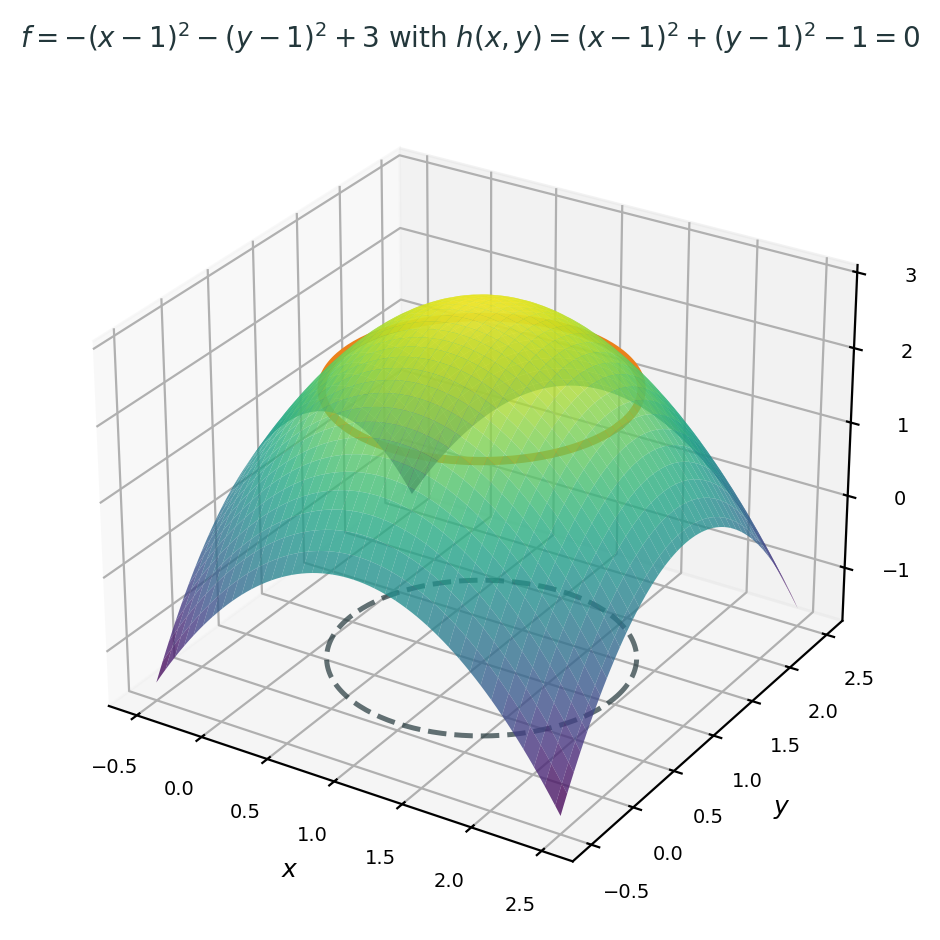
\includegraphics[width=0.60\textwidth]{figures/lagrange_curve_3d.png}
  \end{center}
  
  \small
  Surface $z = f(x,y)$ with constraint curve $h(x,y) = 0$ on the domain.
  
  The optimum occurs where the constraint curve is tangent to a level curve of $f$.
\end{frame}

\begin{frame}{4.3 The tangent argument}
  \small
  At a constrained optimum $\mathbf{x}^*$ on the constraint surface:
  
  \begin{itemize}
    \item Any feasible direction $\mathbf{d}$ (tangent to constraint) satisfies $\nabla h(\mathbf{x}^*) \cdot \mathbf{d} = 0$
    
    \item If $\nabla f(\mathbf{x}^*) \cdot \mathbf{d} \neq 0$, we could move along constraint to increase $f$
    
    \item At optimum, no feasible improving direction exists
  \end{itemize}
  
  \textbf{Conclusion.} $\nabla f(\mathbf{x}^*)$ must be parallel to $\nabla h(\mathbf{x}^*)$.
  
  That is: $\nabla f(\mathbf{x}^*) = -\lambda \nabla h(\mathbf{x}^*)$ for some scalar $\lambda$.
\end{frame}

\begin{frame}{4.3 Lagrangian and first-order conditions}
  \small
  \textbf{Theorem.} At a constrained optimum (with regularity), there exists $\lambda \in \mathbb{R}$ such that
  
  \[
    \nabla f(\mathbf{x}^*) + \lambda \nabla h(\mathbf{x}^*) = \mathbf{0}, \quad h(\mathbf{x}^*) = 0.
  \]
  
  \textbf{Lagrangian.} $\mathcal{L}(\mathbf{x}, \lambda) = f(\mathbf{x}) + \lambda h(\mathbf{x})$.
  
  \begin{itemize}
    \item Stationarity: $\nabla_{\mathbf{x}} \mathcal{L} = \nabla f + \lambda \nabla h = \mathbf{0}$
    
    \item Constraint: $\partial \mathcal{L}/\partial \lambda = h = 0$
  \end{itemize}
  
  $\lambda$ is the \textbf{Lagrange multiplier}.
\end{frame}

\begin{frame}{4.3 Sensitivity without the Lagrangian}
  \small
  Problem: $\max_x f(x)$ subject to $h(x)=c$. At an optimum, $\nabla f(x^*)=\lambda\,\nabla h(x^*)$.
  
  Relax the constraint a little: move to $x^*+dx$ with
  \[
    h(x^*+dx)=c+dc.
  \]
  
  First-order expansion: $\nabla h\cdot dx=dc$. Total differential of the objective: $df=\nabla f\cdot dx$.
  
  Substitute the FOC:
  \[
    df=\nabla f\cdot dx=\lambda\,\nabla h\cdot dx=\lambda\,dc.
  \]
  
  Hence $\displaystyle\frac{dV}{dc}=\lambda$: the multiplier is the sensitivity of $f$ to relaxing the constraint.
\end{frame}

\begin{frame}{4.3 Connect to the Lagrangian}
  \small
  Same problem: $\max_x f(x)$ s.t.\ $h(x)=c$, with $\mathcal{L}(x,\lambda;c)=f(x)+\lambda\bigl(c-h(x)\bigr)$.
  
  Let $V(c)=f(x^*(c))$. Binding constraint $\Rightarrow$ $V(c)=\mathcal{L}(x^*(c),\lambda^*(c);c)$.
  
  Chain rule: FOCs kill $\nabla_x\mathcal{L}\cdot dx^*/dc$ and $(\partial\mathcal{L}/\partial\lambda)\,d\lambda^*/dc$, so
  \[
    \frac{dV}{dc}=\frac{\partial\mathcal{L}}{\partial c}.
  \]
  
  And $\partial\mathcal{L}/\partial c=\lambda^*$ by inspection of $\mathcal{L}$.
  
  \textbf{Summary.} $\displaystyle\frac{dV}{dc}=\frac{\partial\mathcal{L}}{\partial c}=\lambda^*$.
\end{frame}

\QFrame{4.3 Exercise: Cobb--Douglas with budget}
  \small
  \textbf{Exercise.} Maximize $u(x_1, x_2) = x_1^\alpha x_2^{1-\alpha}$ subject to $p_1x_1 + p_2x_2 = w$.
  
  \textbf{Solution.}
  
  \begin{itemize}
    \item Lagrangian: $\mathcal{L} = u + \lambda(w - p_1x_1 - p_2x_2)$
    
    \item FOCs: $\frac{\partial u}{\partial x_1} = \lambda p_1$, $\frac{\partial u}{\partial x_2} = \lambda p_2$
    
    \item Expanding: $\frac{\alpha u}{x_1} = \lambda p_1$, $\frac{(1-\alpha)u}{x_2} = \lambda p_2$
    
    \item Taking ratio: $\frac{\alpha x_2}{(1-\alpha)x_1} = \frac{p_1}{p_2}$
  \end{itemize}
  
  With budget: $p_1x_1 = \alpha w$, $p_2x_2 = (1-\alpha)w$ (constant expenditure shares, Day~1).
  
  From the FOC, $\lambda = \frac{\partial u/\partial x_1}{p_1}$: $\lambda$ is the utility gain from spending one more dollar on $x_1$
  (same for $x_2$ at the optimum).
\end{frame}

\QFrame{4.3 Exercise: Interpreting the multiplier}
  \small
  \textbf{Exercise.} In the Cobb--Douglas solution, compute $\lambda^*$ and interpret it.
  
  \textbf{Solution.} From FOC and $p_1x_1=\alpha w$: $\lambda=u/w$. Plug in demands:
  \[
    \lambda^*=\frac{\alpha^\alpha(1-\alpha)^{1-\alpha}}{p_1^\alpha p_2^{1-\alpha}}.
  \]
  
  In general we only know $\lambda^*=dV/dw$ (shadow price). Here something stronger holds: $\lambda^*=u^*/w=V/w$.
  
  That is CD-specific: MUI equals \emph{average} utility per dollar, not just the marginal.
  
  Since the explicit $\lambda^*$ does not depend on $w$, integrate $dV/dw=\lambda^*$ with $V(0)=0$ to get $V(w)=\lambda^* w$, which is consistent with $\lambda^*=V/w$.
\end{frame}

\begin{frame}{4.3 Why is MUI constant in $w$?}
  \small
  At an optimum, $MRS=p_1/p_2$. For CD, $MRS=\frac{\alpha}{1-\alpha}\frac{x_2}{x_1}$ depends only on the consumption \emph{ratio}.
  
  So $x_1/x_2$ is pinned down by prices alone --- it does not change when $w$ rises.
  
  \textbf{Key intuition.} The mix is fixed; if wealth increases, consumption of each good rises \emph{proportionally}:
  \[
    x^*(w)=w\,x^*(1).
  \]
  
  CD is HD1, so $V(w)=u(w\,x^*(1))=w\,V(1)$, hence $dV/dw=V(1)$ is constant in $w$.
\end{frame}

\THFrame{4.3 Exercise: Cost minimization}
  \small
  \textbf{Exercise.} Minimize $C(q_1, q_2) = r_1q_1 + r_2q_2$ subject to $F(q_1, q_2) = \bar{y}$.
  
  \textbf{Solution.}
  
  \begin{itemize}
    \item Lagrangian: $\mathcal{L} = r_1q_1 + r_2q_2 + \lambda(\bar{y} - F(q_1, q_2))$
    
    \item FOCs: $r_1 = \lambda F_1$, $r_2 = \lambda F_2$ where $F_i = \frac{\partial F}{\partial q_i}$
    
    \item Therefore: $\frac{r_1}{r_2} = \frac{F_1}{F_2}$
  \end{itemize}
  
  The input price ratio equals the marginal rate of technical substitution.
  
  Same logic: $\lambda = dC^*/d\bar{y}$, the marginal cost of relaxing the output constraint.
\end{frame}

%==============================================================================
\section{4.4 --- Envelope Theorem}
%==============================================================================

\begin{frame}{4.4 Value functions and parameters}
  \small
  Economic problems depend on parameters: prices, income, technology.
  
  \textbf{Value function.} $V(\theta) = \max_{\mathbf{x}} f(\mathbf{x}; \theta)$ subject to constraints.
  
  We want to know: how does the optimal value change when $\theta$ shifts?
  
  \textbf{Key question:} Do we need to account for how $\mathbf{x}^*(\theta)$ changes?
\end{frame}

\begin{frame}{4.4 Unconstrained envelope theorem}
  \small
  \textbf{Theorem.} For $V(\theta) = \max_{\mathbf{x}} f(\mathbf{x}; \theta)$ with optimizer $\mathbf{x}^*(\theta)$:
  
  \[
    \frac{dV}{d\theta} = \frac{\partial f}{\partial \theta}\Big|_{\mathbf{x}=\mathbf{x}^*(\theta)}.
  \]
  
  \textbf{Proof.} By chain rule:
  
  \[
    \frac{dV}{d\theta} = \underbrace{\nabla_{\mathbf{x}}f \cdot \frac{d\mathbf{x}^*}{d\theta}}_{=0 \text{ by FOC}} + \frac{\partial f}{\partial \theta} = \frac{\partial f}{\partial \theta}.
  \]
  
  \textbf{Intuition.} First-order gains from adjusting $\mathbf{x}$ vanish at optimum. Only direct effects of $\theta$ on $f$ matter.
\end{frame}

\begin{frame}{4.4 Constrained envelope theorem}
  \small
  With constraints and Lagrangian $\mathcal{L} = f + \sum \lambda_k h_k$:
  
  \[
    \frac{dV}{d\theta} = \frac{\partial \mathcal{L}}{\partial \theta}\Big|_{(\mathbf{x}^*, \boldsymbol{\lambda}^*)}.
  \]
  
  \textbf{Proof.} Differentiate $V(\theta) = \mathcal{L}(\mathbf{x}^*(\theta), \boldsymbol{\lambda}^*(\theta); \theta)$:
  
  \begin{itemize}
    \item Terms with $\partial \mathbf{x}^*/\partial \theta$ vanish by stationarity ($\nabla_{\mathbf{x}}\mathcal{L}=0$)
    
    \item Terms with $\partial \lambda_k/\partial \theta$ vanish by constraints ($h_k = 0$)
  \end{itemize}
  
  Shadow prices absorb the effect of constraint relaxation.
\end{frame}

\QFrame{4.4 Exercise: Profit function}
  \small
  \textbf{Exercise.} For $\pi^*(p) = \max_{q \geq 0} pq - C(q)$, find $\frac{d\pi^*}{dp}$.
  
  \textbf{Solution by envelope.}
  
  \begin{itemize}
    \item $\frac{d\pi^*}{dp} = \frac{\partial(pq - C(q))}{\partial p}\big|_{q^*} = q^*(p)$
    
    \item The supply function!
  \end{itemize}
  
  \textbf{Verify explicitly.}
  
  \begin{itemize}
    \item FOC: $p = C'(q^*)$ defines $q^*(p)$
    
    \item $\pi^*(p) = pq^*(p) - C(q^*(p))$
    
    \item $\frac{d\pi^*}{dp} = q^* + p\frac{dq^*}{dp} - C'(q^*)\frac{dq^*}{dp} = q^* + \underbrace{(p - C'(q^*))}_{=0}\frac{dq^*}{dp} = q^*$
  \end{itemize}
  
  Envelope gives this directly without computing $\frac{dq^*}{dp}$.
\end{frame}

\begin{frame}{4.4 Budget set and indirect utility}
  \small
  \textbf{Budget set.} $B(p,w)=\{\mathbf{x}\geq\mathbf{0}:\,p\cdot\mathbf{x}\leq w\}$.
  
  \textbf{Consumer problem.} $\max_{\mathbf{x}} u(\mathbf{x})$ subject to $\mathbf{x}\in B(p,w)$.
  
  Let $\mathbf{x}^*(p,w)$ be the Marshallian demand (optimizer).
  
  \textbf{Indirect utility.} The value function of this problem:
  \[
    V(p,w)=\max_{\mathbf{x}\in B(p,w)} u(\mathbf{x})=u\bigl(\mathbf{x}^*(p,w)\bigr).
  \]
  
  $V$ is maximized utility as a function of prices and wealth --- not of the goods themselves.
\end{frame}

\QFrame{4.4 Exercise: Roy's identity}
  \small
  \textbf{Exercise.} Show that
  \[
    \frac{\partial V/\partial p_i}{\partial V/\partial w}=-x_i^*(p,w).
  \]

  \textbf{Solution.} Envelope: $\partial V/\partial p_i=-\lambda^* x_i^*$, $\partial V/\partial w=\lambda^*$.
  Ratio:
  \[
    \frac{-\lambda^* x_i^*}{\lambda^*}=-x_i^*.
  \]
  
  So Marshallian demand is recovered from $V$ without re-solving the consumer problem.
\end{frame}

\begin{frame}{4.4 How $p_i$ changes $V$: two channels}
  \small
  Why is $\partial V/\partial p_i=-\lambda^* x_i^*$? Write $V$ via
  $\mathcal{L}=u(\mathbf{x})+\lambda(w-p\cdot\mathbf{x})$, so
  $V=\mathcal{L}\bigl(\mathbf{x}^*,\lambda^*;p,w\bigr)$.
  
  Differentiate in $p_i$:
  \[
    \frac{\partial V}{\partial p_i}
    =\underbrace{\nabla_{\mathbf{x}}\mathcal{L}\cdot\frac{\partial\mathbf{x}^*}{\partial p_i}}_{=0\text{ (FOC)}}
    +\underbrace{\frac{\partial\mathcal{L}}{\partial\lambda}\,\frac{\partial\lambda^*}{\partial p_i}}_{=0\text{ (budget binds)}}
    +\underbrace{\frac{\partial\mathcal{L}}{\partial p_i}}_{=-\lambda^* x_i^*}.
  \]
  
  \textbf{Two channels.}
  \begin{itemize}
    \item Fix $\mathbf{x}$: higher $p_i$ costs $x_i^*$ more dollars for the same basket --- valued at $\lambda^*$ utils each.
    \item Reoptimize $\mathbf{x}^*$ (and $\lambda^*$): first-order effect is zero at an optimum.
  \end{itemize}
\end{frame}

%==============================================================================
\section{4.5 --- Inequality Constraints: Farkas Lemma and KKT}
%==============================================================================

\begin{frame}{4.5 Problems with inequality constraints}
  \small
  \textbf{Problem.} Maximize $f(\mathbf{x})$ subject to $g_j(\mathbf{x}) \leq 0$ for $j=1,\ldots,m$.
  
  \textbf{Binding vs. slack constraints.}
  
  \begin{itemize}
    \item \textbf{Binding (active):} $g_j(\mathbf{x}^*) = 0$ --- constraint holds with equality
    
    \item \textbf{Slack (inactive):} $g_j(\mathbf{x}^*) < 0$ --- constraint not tight
  \end{itemize}
  
  Only binding constraints matter for local optimality.
  
  Slack constraints can be ignored locally.
\end{frame}

\begin{frame}{4.5 Feasible directions and the cone}
  \small
  At a boundary point with active constraints, \textbf{feasible directions} form a convex cone:
  
  \[
    D = \{\mathbf{d} : \nabla g_j(\mathbf{x}^*) \cdot \mathbf{d} \leq 0 \text{ for all active } j\}.
  \]
  
  A direction $\mathbf{d}$ is \textbf{improving} if $\nabla f \cdot \mathbf{d} > 0$ (increases objective).
  
  For a local maximum: no feasible direction can be improving.
\end{frame}

\begin{frame}{4.5 Geometric intuition of Farkas lemma}
  \begin{center}
    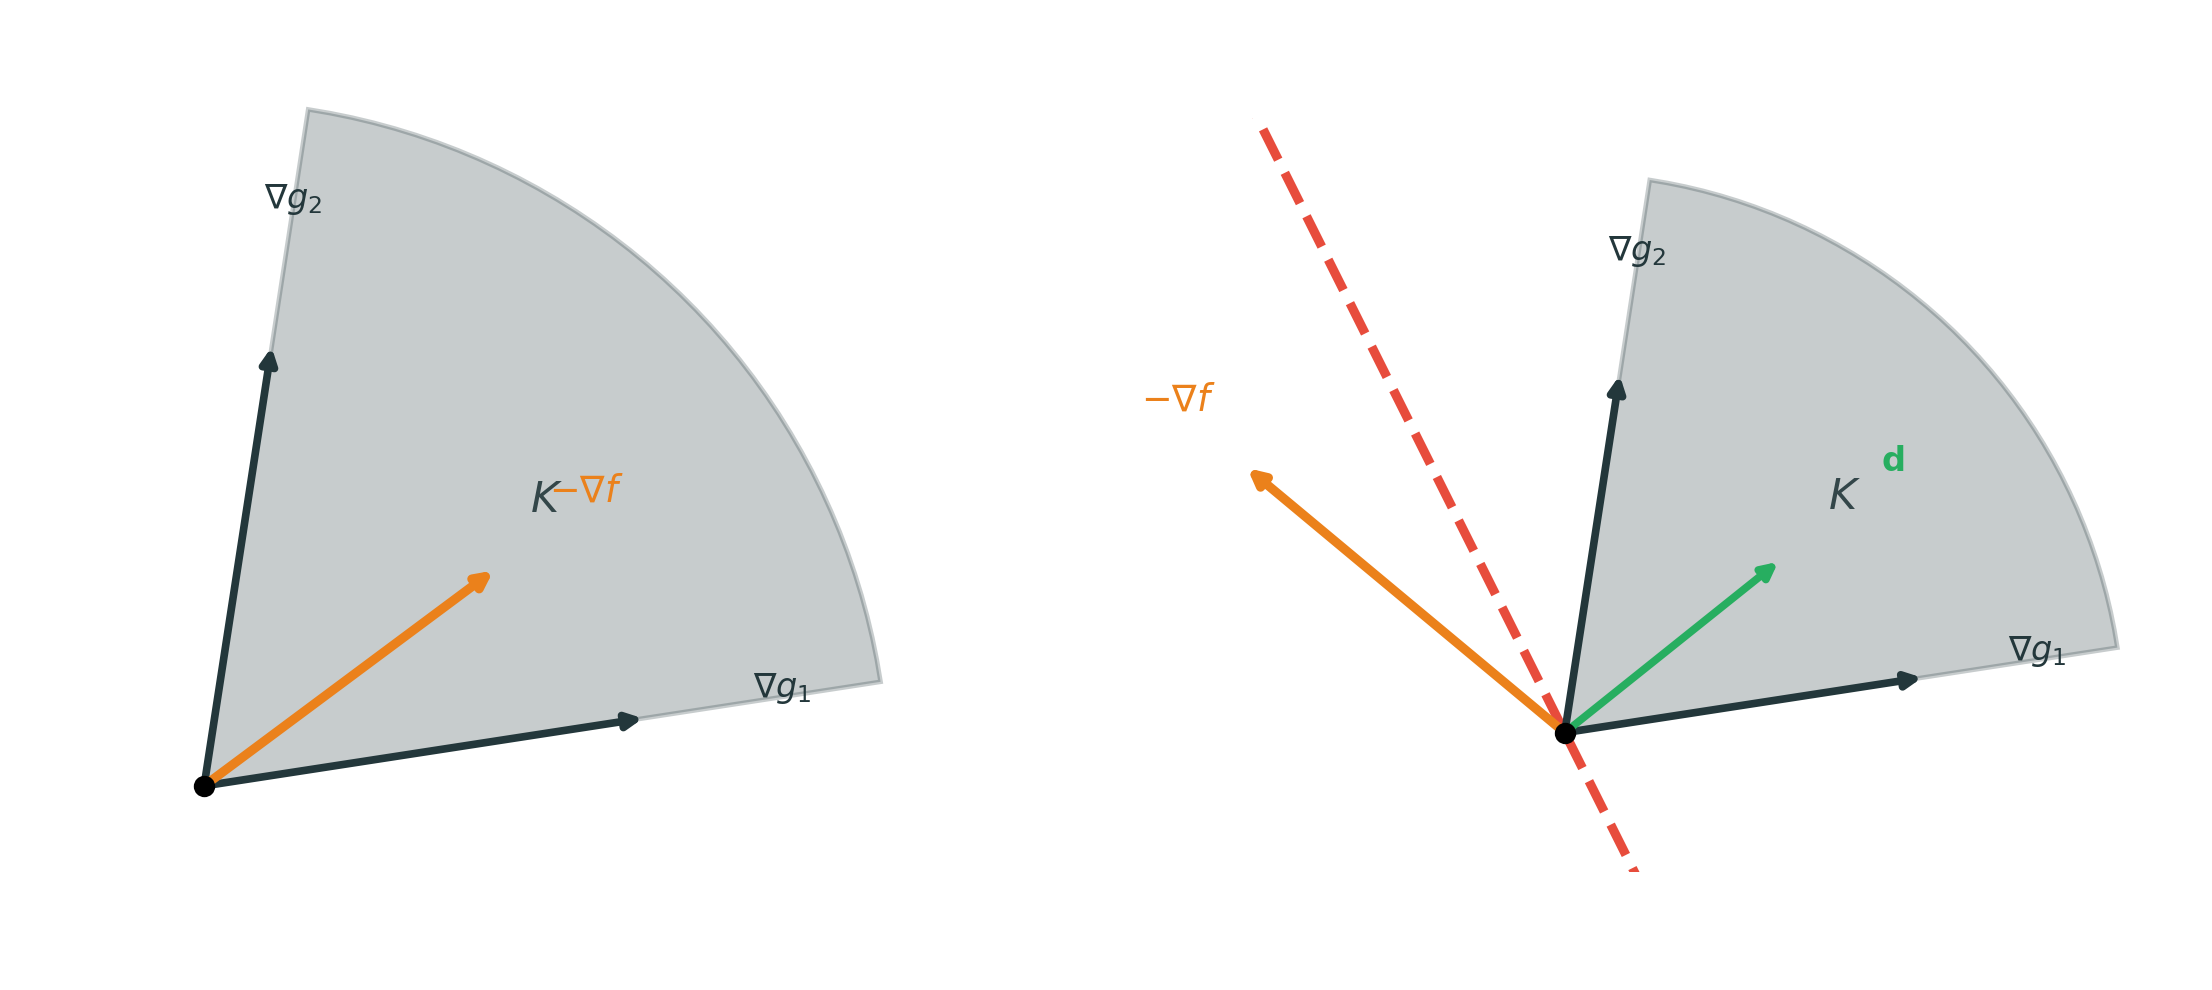
\includegraphics[width=0.95\textwidth]{figures/farkas_simple.png}
  \end{center}
\end{frame}

\begin{frame}{4.5 Statement of Farkas lemma}
  \small
  \textbf{Farkas Lemma (purely geometric).}
  
  Let $K$ be a closed convex cone and $\mathbf{y}$ a vector. Either:
  
  \begin{enumerate}
    \item $\mathbf{y} \in K$: the vector lies in the cone
    
    \item $\mathbf{y} \notin K$: there exists a separating hyperplane with normal $\mathbf{d}$ such that
    
    \begin{itemize}
      \item $\mathbf{k} \cdot \mathbf{d} \leq 0$ for all $\mathbf{k} \in K$ (cone on one side)
      
      \item $\mathbf{y} \cdot \mathbf{d} > 0$ (vector on the other side)
    \end{itemize}
  \end{enumerate}
  
  The hyperplane strictly separates the cone from the vector.
\end{frame}

\begin{frame}{4.5 Applying Farkas to optimization}
  \small
  Maximize $f$ subject to $g_j\leq 0$. Let $K=\mathrm{cone}\{\nabla g_j:g_j\text{ active}\}$.
  
  \textbf{Farkas, applied:} either $\nabla f\in K$, or there is a feasible improving direction.
  
  \textbf{Case 1 (optimal).} $\nabla f\in K$: $\nabla f$ is a nonnegative combination of the active $\nabla g_j$.
  With $\mathcal{L}=f+\sum_j\lambda_j g_j$, this is exactly
  \[
    \nabla f+\sum_j\lambda_j\nabla g_j=\mathbf{0}\quad\text{for some }\lambda_j\leq 0.
  \]
  (Why $\leq 0$? Stationarity gives $\nabla f=-\sum\lambda_j\nabla g_j$; to lie in $K$ we need $-\lambda_j\geq 0$.)
  
  \textbf{Case 2 (not optimal).} $\nabla f\notin K$: some $\mathbf{d}$ with $\nabla g_j\cdot\mathbf{d}\leq 0$ (feasible) and $\nabla f\cdot\mathbf{d}>0$ (improving).
\end{frame}

\begin{frame}{4.5 Inequality problem with multipliers}
  \small
  At an optimum, Case 2 is ruled out --- so Case 1 holds:
  
  \[
    \nabla f(\mathbf{x}^*) + \sum_{\text{active}} \lambda_j \nabla g_j(\mathbf{x}^*) = \mathbf{0}, \quad \lambda_j \leq 0.
  \]
  
  \textbf{Binding:} $\lambda_j<0$ possible (these constraints bite).
  
  \textbf{Slack:} $\lambda_j=0$ (inactive constraints drop out of $\mathcal{L}$).
  
  Same $\lambda$ as in the Lagrangian --- no extra symbols.
\end{frame}

\begin{frame}{4.5 KKT conditions}
  \small
  \textbf{Theorem (KKT necessary conditions).} At a local maximum (with constraint qualification), there exist multipliers $\lambda_j$ such that:
  
  \begin{enumerate}
    \item \textbf{Stationarity:} $\nabla f(\mathbf{x}^*) + \sum_j \lambda_j \nabla g_j(\mathbf{x}^*) = \mathbf{0}$
    
    \item \textbf{Primal feasibility:} $g_j(\mathbf{x}^*) \leq 0$ for all $j$
    
    \item \textbf{Dual feasibility:} $\lambda_j \leq 0$ (for $g_j \leq 0$, max problem, $\mathcal{L}=f+\sum\lambda_j g_j$)
    
    \item \textbf{Complementary slackness:} $\lambda_j g_j(\mathbf{x}^*) = 0$
  \end{enumerate}
  
  CS says: multiplier is zero for slack constraints ($g_j < 0 \Rightarrow \lambda_j = 0$).
  
  Stationarity says: $\nabla f$ is a nonnegative combination of active $\nabla g_j$ (since $\lambda_j\leq 0$).
\end{frame}

\begin{frame}{4.5 Sign convention summary}
  \small
  With $\mathcal{L} = f + \sum_j \lambda_j g_j$ (always $+$):
  
  \begin{center}
    \begin{tabular}{@{}lll@{}}
      \toprule
      Problem & Constraint & $\lambda$ sign \\
      \midrule
      $\max f$ & $g \leq 0$ & $\lambda \leq 0$ \\
      $\max f$ & $g \geq 0$ & $\lambda \geq 0$ \\
      $\min f$ & $g \leq 0$ & $\lambda \geq 0$ \\
      $\min f$ & $g \geq 0$ & $\lambda \leq 0$ \\
      \bottomrule
    \end{tabular}
  \end{center}
  
  \textbf{Memory rule (multiply signs).}
  Assign: max $=+$, min $=-\,;$ $\leq=-\,;$ $\geq=+$.
  The sign of $\lambda$ is the product:
  \[
    \underbrace{\mathrm{max}/\!\mathrm{min}}_{\pm}
    \times
    \underbrace{g\,\leq/\!\geq}_{\pm}
    \;=\;
    \mathrm{sign}(\lambda).
  \]
  Example: max and $g\leq 0$ $\Rightarrow$ $(+)\times(-)=-$ $\Rightarrow$ $\lambda\leq 0$.
\end{frame}

\QFrame{4.5 Exercise: Budget with nonnegativity}
  \small
  \textbf{Exercise.} Maximize $u(x_1,x_2)=x_1 x_2$ subject to $x_1+x_2\leq 1$, $x_1\geq 0$, $x_2\geq 0$.

  $g_1=x_1+x_2-1\leq 0$, $g_2=-x_1\leq 0$, $g_3=-x_2\leq 0$, $\lambda_j\leq 0$.
  \[
    \mathcal{L}=x_1 x_2+\lambda_1(x_1+x_2-1)+\lambda_2(-x_1)+\lambda_3(-x_2).
  \]
  Stationarity: $x_2+\lambda_1-\lambda_2=0$,\quad $x_1+\lambda_1-\lambda_3=0$.\\
  CS: $\lambda_1(x_1+x_2-1)=0$,\quad $\lambda_2 x_1=0$,\quad $\lambda_3 x_2=0$.

  \textbf{Method.} In general each $g_j$ binds or not $\Rightarrow$ $2^3=8$ patterns.
  We illustrate three: interior max, a corner that fails KKT, and a point where KKT holds but is not a max.
\end{frame}

\QFrame{4.5 Case: Only budget binds}
  \small
  Stationarity: $x_2+\lambda_1-\lambda_2=0$,\quad $x_1+\lambda_1-\lambda_3=0$.\\
  CS: $\lambda_1(x_1+x_2-1)=0$,\quad $\lambda_2 x_1=0$,\quad $\lambda_3 x_2=0$
  \quad ($\lambda_j\leq 0$).

  \textbf{Case.} $x_1+x_2=1$ and $x_1,x_2>0$ $\Rightarrow$ $\lambda_2=\lambda_3=0$.

  \begin{itemize}
    \item Stationarity: $x_2+\lambda_1=0$, $x_1+\lambda_1=0$ $\Rightarrow$ $x_1=x_2=-\lambda_1$

    \item Budget: $x_1+x_2=1$ $\Rightarrow$ $x_1=x_2=\tfrac12$, $\lambda_1=-\tfrac12\leq 0$
  \end{itemize}

  KKT holds with $u=\tfrac14$. This is the maximizer.
\end{frame}

\QFrame{4.5 Case: Budget + one axis}
  \small
  Stationarity: $x_2+\lambda_1-\lambda_2=0$,\quad $x_1+\lambda_1-\lambda_3=0$.\\
  CS: $\lambda_1(x_1+x_2-1)=0$,\quad $\lambda_2 x_1=0$,\quad $\lambda_3 x_2=0$
  \quad ($\lambda_j\leq 0$).

  \textbf{Case.} Budget binds and $x_1=0$, $x_2$ slack: $(0,1)$.
  Then $g_3$ slack $\Rightarrow$ $\lambda_3=0$.

  \begin{itemize}
    \item Stationarity in $x_2$: $\lambda_1=0$

    \item Stationarity in $x_1$: $1-\lambda_2=0$ $\Rightarrow$ $\lambda_2=1>0$
  \end{itemize}

  Violates $\lambda_2\leq 0$ $\Rightarrow$ \textbf{not KKT} $\Rightarrow$ $(0,1)$ cannot be optimal.
  (Same for $(1,0)$ by symmetry.)
\end{frame}

\QFrame{4.5 Case: Both axes bind, KKT but not max}
  \small
  Stationarity: $x_2+\lambda_1-\lambda_2=0$,\quad $x_1+\lambda_1-\lambda_3=0$.\\
  CS: $\lambda_1(x_1+x_2-1)=0$,\quad $\lambda_2 x_1=0$,\quad $\lambda_3 x_2=0$
  \quad ($\lambda_j\leq 0$).

  \textbf{Case.} $x_1=x_2=0$ (both nonnegativity bind), budget slack.

  CS $\Rightarrow$ $\lambda_1=0$. Stationarity $\Rightarrow$ $\lambda_2=\lambda_3=0$.

  KKT holds, but $u(0,0)=0<\tfrac14=u(\tfrac12,\tfrac12)$.

  So KKT is necessary (under CQ), not sufficient: must still compare objective values.
\end{frame}

\QFrame{4.5 Exercise: Cost minimization}
  \small
  \textbf{Exercise.} A firm chooses inputs $z=(z_1,z_2)$ to produce at least $\bar{z}$ units
  with technology $f(z)=z_1+z_2$ (perfect substitutes). Input prices are $p=(p_1,p_2)>0$.
  \[
    \min_{z\geq 0}\; p\cdot z \quad\text{s.t.}\quad z_1+z_2\geq \bar{z}.
  \]

  \textbf{Setup.} Write $g_1=\bar{z}-z_1-z_2\leq 0$, $g_2=-z_1\leq 0$, $g_3=-z_2\leq 0$.
  For a \emph{min} problem with $g_j\leq 0$: $\lambda_j\geq 0$.
  \[
    \mathcal{L}=p_1 z_1+p_2 z_2+\lambda_1(\bar{z}-z_1-z_2)+\lambda_2(-z_1)+\lambda_3(-z_2).
  \]
  Stationarity: $p_1-\lambda_1-\lambda_2=0$,\quad $p_2-\lambda_1-\lambda_3=0$.\\
  CS: $\lambda_1(\bar{z}-z_1-z_2)=0$,\quad $\lambda_2 z_1=0$,\quad $\lambda_3 z_2=0$.
\end{frame}

\QFrame{4.5 Cost min: equal prices vs.\ corner}
  \small
  Stationarity: $p_1=\lambda_1+\lambda_2$,\quad $p_2=\lambda_1+\lambda_3$.\\
  CS: $\lambda_1(\bar{z}-z_1-z_2)=0$,\quad $\lambda_2 z_1=0$,\quad $\lambda_3 z_2=0$
  \quad ($\lambda_j\geq 0$).

  \textbf{Interior in both inputs} ($z_1,z_2>0$). Then $\lambda_2=\lambda_3=0$, so $p_1=p_2=\lambda_1$.
  Output binds: $z_1+z_2=\bar{z}$. Any split works iff $p_1=p_2$.

  \textbf{If $p_1<p_2$.} Cannot have $\lambda_2=\lambda_3=0$. Check the cases with a positive multiplier:

  \begin{itemize}
    \item $\lambda_2>0$: CS $\Rightarrow$ $z_1=0$, so $z_2=\bar{z}$. Then $\lambda_3=0$, $\lambda_1=p_2$,
      $\lambda_2=p_1-p_2<0$. Violates $\lambda_2\geq 0$. \textbf{Fails}.

    \item $\lambda_3>0$: CS $\Rightarrow$ $z_2=0$, so $z_1=\bar{z}$. Then $\lambda_2=0$, $\lambda_1=p_1$,
      $\lambda_3=p_2-p_1>0$. \textbf{Works} (use only the cheaper input).
  \end{itemize}
\end{frame}

%==============================================================================
\section{4.6 --- Why Equality Multipliers Are Unrestricted}
%==============================================================================

\begin{frame}{4.6 Key intuition: one-sided vs.\ two-sided wall}
  \footnotesize
  \textbf{Inequality} $g(\mathbf{x})\leq 0$: a \textbf{one-sided wall}.
  Feasible moves: $\nabla g\cdot\mathbf{d}\leq 0$.
  For a max with one active $g$ and $\mathcal{L}=f+\lambda g$:

  \begin{enumerate}
    \item \textbf{Binding + stationarity} $\Rightarrow$ $\nabla f$ on the
      \emph{same line} as $\nabla g$: $\nabla f=-\lambda\nabla g$
      (same or opposite).
    \item Binding needs $\nabla f\cdot\nabla g>0$ $\Rightarrow$ same way
      $\Rightarrow$ $\lambda<0$.
    \item If $\lambda>0$, $\lambda g$ rewards raising $g$ (violate $g\leq 0$).
      $\lambda<0$ holds that incentive back on the bound.
  \end{enumerate}

  \textbf{Key difference.} When binding: inequality --- you know which way
  raises $f$ (along $\nabla g$, into the forbidden side);
  equality --- you do not (with or against $\nabla h$ may raise or lower $f$).
  So equality $\lambda$ is unrestricted.
\end{frame}

\begin{frame}{4.6 The combined Lagrangian}
  \small
  For problems with both equalities and inequalities:
  \[
    \mathcal{L} = f + \underbrace{\sum_k \lambda_k h_k}_{\text{equality (two-sided)}} + \underbrace{\sum_j \lambda_j g_j}_{\text{inequality (one-sided)}}.
  \]

  \textbf{Sign convention} (max problem):

  \begin{center}
    \begin{tabular}{@{}ll@{}}
      \toprule
      Multiplier & Sign rule \\
      \midrule
      Equality $\lambda_k$ & unrestricted (two-sided wall) \\
      Inequality $\lambda_j$ & $\lambda_j \leq 0$ if $g_j \leq 0$; $\lambda_j \geq 0$ if $g_j \geq 0$ \\
      \bottomrule
    \end{tabular}
  \end{center}

  \textbf{Short rule.} Sign of $\lambda$ $=$ (max $+\,/$ min $-$) $\times$ ($g\geq 0$ $+\,/$ $g\leq 0$ $-$).
\end{frame}

%==============================================================================
\appendix
%==============================================================================

\begin{frame}{Appendix \InterestOnly}
  \footnotesize
  \textbf{Additional proofs and extensions} (same order as main text):
  
  \begin{enumerate}
    \item \hyperlink{appendix:soc_1d}{A.1} Unconstrained optimization: FOC and SOC (1D)
    \item \hyperlink{appendix:concave_12}{A.2} Concavity: $(1)\Leftrightarrow(2)$
    \item \hyperlink{appendix:concave_23}{A.3} Concavity: $(2)\Leftrightarrow(3)$
    \item \hyperlink{appendix:multivariate_concave}{A.4} Proof: multivariate $(2)\Leftrightarrow(3)$
    \item \hyperlink{appendix:multivariate_soc}{A.5} Multivariate SOC
    \item \hyperlink{appendix:logconcave}{A.6} Log-concavity
    \item \hyperlink{appendix:exercises}{A.7} Additional exercises
  \end{enumerate}
\end{frame}

\hypertarget{appendix:soc_1d}{}
\begin{frame}{A.1 Proof: First-Order Condition (1D)}
  \small
  \InterestOnly
  
  \textbf{Theorem.} If $x^*$ is an interior local maximum and $f$ is differentiable at $x^*$, then $f'(x^*) = 0$.
  
  \textbf{Proof.}
  
  \begin{itemize}
    \item If $f'(x^*) > 0$: then $f(x^* + h) > f(x^*)$ for small $h > 0$, contradiction
    
    \item If $f'(x^*) < 0$: then $f(x^* + h) > f(x^*)$ for small $h < 0$, contradiction
  \end{itemize}
\end{frame}

\begin{frame}{A.1 Proof: Necessary SOC (1D)}
  \small
  \InterestOnly
  
  \textbf{Theorem.} If $x^*$ is an interior local maximum and $f \in C^2$, then $f''(x^*) \leq 0$.
  
  \textbf{Proof.} Suppose $f''(x^*) > 0$. Taylor at $x^*$:
  \[
    f(x^* + h)
    =
    f(x^*) + \tfrac12 f''(x^*) h^2 + o(h^2).
  \]
  
  \begin{itemize}
    \item For small $h \neq 0$, the quadratic term dominates the remainder
    
    \item Since $f''(x^*) > 0$, we get $f(x^* + h) > f(x^*)$ --- contradiction
    
    \item Therefore $f''(x^*) \leq 0$
  \end{itemize}
\end{frame}

\begin{frame}{A.1 Proof: Sufficient SOC (1D)}
  \small
  \InterestOnly
  
  \textbf{Theorem.} If $f'(x^*) = 0$ and $f''(x^*) < 0$, then $x^*$ is a strict local maximum.
  
  \textbf{Proof.} Taylor expansion around $x^*$:
  \[
    f(x^* + h) = f(x^*) + \underbrace{f'(x^*)}_{=0} h + \tfrac12 f''(x^*) h^2 + o(h^2).
  \]
  
  \begin{itemize}
    \item For small $h$, the $h^2$ term dominates the remainder
    
    \item Since $f''(x^*) < 0$, we have $f(x^* + h) < f(x^*)$ for small $h \neq 0$
  \end{itemize}
\end{frame}

\hypertarget{appendix:concave_12}{}
\begin{frame}{A.2 Proof $(1) \Rightarrow (2)$}
  \small
  \InterestOnly
  
  \textbf{Proof.} Fix $x$ and $y > x$. Set $h = y - x > 0$.
  
  For $t \in (0,1]$, the point on the segment is
  \[
    x + th = (1-t)x + ty.
  \]
  
  \begin{itemize}
    \item By concavity: $f(x+th) \geq (1-t)f(x) + tf(y)$
    
    \item Rearrange: $f(x+th) - f(x) \geq t(f(y)-f(x))$
    
    \item Divide by $th > 0$:
    \[
      \frac{f(x+th)-f(x)}{th} \geq \frac{f(y)-f(x)}{y-x}.
    \]
    
    \item Let $t \to 0^+$: $f'(x) \geq \dfrac{f(y)-f(x)}{y-x}$
    
    \item So $f(y) \leq f(x) + f'(x)(y-x)$. The case $y < x$ is similar
  \end{itemize}
\end{frame}

\begin{frame}{A.2 Proof $(2) \Rightarrow (1)$}
  \small
  \InterestOnly
  
  \textbf{Proof.} Fix $x$, $y$, and $\lambda \in [0,1]$. Let $u=\lambda x+(1-\lambda)y$.
  
  \begin{itemize}
    \item Tangent at $u$: $f(x) \leq f(u)+f'(u)(x-u)$ and $f(y) \leq f(u)+f'(u)(y-u)$
    
    \item Weight by $(1-\lambda)$ and $\lambda$, then add:
    \[
      (1-\lambda)f(x)+\lambda f(y)
      \leq f(u) + f'(u)\big[(1-\lambda)(x-u)+\lambda(y-u)\big].
    \]
    
    \item The bracket is $0$ because $u=\lambda x+(1-\lambda)y$
    
    \item So $(1-\lambda)f(x)+\lambda f(y) \leq f(u)=f(\lambda x+(1-\lambda)y)$
  \end{itemize}
\end{frame}

\hypertarget{appendix:concave_23}{}
\begin{frame}{A.3 Proof $(2) \Rightarrow (3)$}
  \small
  \InterestOnly
  
  \textbf{Proof.} Since $(1) \Leftrightarrow (2)$, use the chord form. From concavity with endpoints $x+h$, $x-h$ and $\lambda=\tfrac12$:
  \[
    f(x) = f\!\left(\tfrac12(x+h)+\tfrac12(x-h)\right)
    \geq \tfrac12 f(x+h) + \tfrac12 f(x-h).
  \]
  So $f(x+h) + f(x-h) \leq 2f(x)$ for all $h > 0$.
  
  Rearrange and divide by $h > 0$:
  \[
    \frac{f(x+h) - f(x)}{h} \leq \frac{f(x) - f(x-h)}{h}.
  \]
  
  Bring to one side and divide by $h$ again:
  \[
    \frac{f(x+h) - 2f(x) + f(x-h)}{h^2} \leq 0.
  \]
  
  Let $h \to 0$: limit is $f''(x) \leq 0$.
  
  \vfill
  \hfill\hyperlink{appendix:rigorous_concave}{\scriptsize Rigorous version: next slides}
\end{frame}

\begin{frame}{A.3 Proof $(3) \Rightarrow (2)$}
  \small
  \InterestOnly
  
  \textbf{Proof.} Fix any $x$ and $y$. Taylor around $x$:
  \[
    f(y)
    =
    f(x) + f'(x)(y-x)
    + \frac{1}{2}f''(\xi)(y-x)^2,
  \]
  where $\xi$ lies between $x$ and $y$.
  
  \begin{itemize}
    \item Since $f''(\xi) \leq 0$ and $(y-x)^2 \geq 0$, the second-order term is $\leq 0$
    
    \item Therefore: $f(y) \leq f(x) + f'(x)(y-x)$
    
    \item This is the tangent characterization of concavity
  \end{itemize}
\end{frame}

\hypertarget{appendix:rigorous_concave}{}
\begin{frame}{A.3 Rigorous proof: concave $\Rightarrow$ $f'' \leq 0$ (I)}
  \small
  \InterestOnly
  
  \textbf{Theorem.} If $f$ is concave and $f \in C^2$, then $f''(x) \leq 0$ for all $x$.
  
  \textbf{Rigorous proof using Taylor expansion with remainder.}
  
  From concavity with endpoints $x+h$, $x-h$ and $\lambda=\tfrac12$:
  \[
    f(x) \geq \tfrac12 f(x+h) + \tfrac12 f(x-h)
    \quad\Leftrightarrow\quad
    f(x+h) + f(x-h) \leq 2f(x).
  \]
  
  Taylor expansions around $x$:
  \begin{align*}
    f(x+h) &= f(x) + f'(x)h + \frac{1}{2}f''(x)h^2 + \frac{f'''(\xi_1)}{6}h^3 \\
    f(x-h) &= f(x) - f'(x)h + \frac{1}{2}f''(x)h^2 - \frac{f'''(\xi_2)}{6}h^3
  \end{align*}
  where $\xi_1$ lies between $x$ and $x+h$, and $\xi_2$ between $x-h$ and $x$.
\end{frame}

\begin{frame}{A.3 Rigorous proof: concave $\Rightarrow$ $f'' \leq 0$ (II)}
  \small
  \InterestOnly
  
  Adding the two Taylor expansions:
  \[
    f(x+h) + f(x-h) = 2f(x) + f''(x)h^2 + \frac{f'''(\xi_1) - f'''(\xi_2)}{6}h^3.
  \]
  
  \begin{itemize}
    \item By concavity: $f''(x)h^2 + \frac{f'''(\xi_1) - f'''(\xi_2)}{6}h^3 \leq 0$
    
    \item Divide by $h^2 > 0$:
    \[
      f''(x) + \frac{f'''(\xi_1) - f'''(\xi_2)}{6}h \leq 0
    \]
    
    \item Let $h \to 0$: third-order terms vanish, leaving $f''(x) \leq 0$
  \end{itemize}
\end{frame}

\hypertarget{appendix:multivariate_concave}{}
\begin{frame}{A.4 Proof $(3) \Rightarrow (2)$}
  \small
  \InterestOnly
  
  Proof of $(2)\Leftrightarrow(3)$ for multivariate concavity.
  
  \textbf{Proof.} Taylor around $\mathbf{x}$:
  \[
    f(\mathbf{x}+\mathbf{h})
    =
    f(\mathbf{x}) + \nabla f(\mathbf{x})^\top \mathbf{h}
    + \frac{1}{2}\mathbf{h}^\top H_f(\boldsymbol{\xi})\mathbf{h},
  \]
  where $\boldsymbol{\xi}$ lies on the segment from $\mathbf{x}$ to $\mathbf{x}+\mathbf{h}$.
  
  \begin{itemize}
    \item If $H_f(\boldsymbol{\xi})$ is NSD, then $\mathbf{h}^\top H_f(\boldsymbol{\xi})\mathbf{h} \leq 0$
    
    \item So $f(\mathbf{x}+\mathbf{h}) \leq f(\mathbf{x}) + \nabla f(\mathbf{x})^\top \mathbf{h}$
    
    \item Writing $\mathbf{y}=\mathbf{x}+\mathbf{h}$ gives the tangent characterization
  \end{itemize}
\end{frame}

\begin{frame}{A.4 Proof $(2) \Rightarrow (3)$}
  \small
  \InterestOnly
  
  \textbf{Proof.} Fix $\mathbf{x}$ and any $\mathbf{h} \in \mathbb{R}^n$. By concavity with endpoints $\mathbf{x}+\mathbf{h}$, $\mathbf{x}-\mathbf{h}$ and $\lambda=\tfrac12$:
  \[
    f(\mathbf{x}) \geq \tfrac12 f(\mathbf{x}+\mathbf{h}) + \tfrac12 f(\mathbf{x}-\mathbf{h}).
  \]
  
  \begin{itemize}
    \item Taylor expand $f(\mathbf{x}\pm\mathbf{h})$ around $\mathbf{x}$ and add
    
    \item The first-order terms cancel; the remainder gives
    \[
      \mathbf{h}^\top H_f(\mathbf{x})\mathbf{h} + o(\|\mathbf{h}\|^2) \leq 0
    \]
    
    \item Let $\|\mathbf{h}\| \to 0$: $\mathbf{h}^\top H_f(\mathbf{x})\mathbf{h} \leq 0$ for all $\mathbf{h}$
    
    \item So $H_f(\mathbf{x})$ is NSD
  \end{itemize}
\end{frame}

\hypertarget{appendix:multivariate_soc}{}
\begin{frame}{A.5 Proof: Necessary SOC (multivariate)}
  \small
  \InterestOnly
  
  \textbf{Theorem.} If $\mathbf{x}^*$ is an interior local maximum and $f \in C^2$, then $H_f(\mathbf{x}^*)$ is negative semidefinite.
  
  \textbf{Proof.} Suppose some eigenvalue $\lambda > 0$ with unit eigenvector $\mathbf{v}$ ($H_f(\mathbf{x}^*)\mathbf{v}=\lambda\mathbf{v}$, $\|\mathbf{v}\|=1$). Taylor at $\mathbf{x}^*$:
  \[
    f(\mathbf{x}^* + t\mathbf{v})
    =
    f(\mathbf{x}^*) + \tfrac12 t^2 \mathbf{v}^\top H_f(\mathbf{x}^*)\mathbf{v} + o(t^2).
  \]
  
  \begin{itemize}
    \item Since $\mathbf{v}$ is an eigenvector: $\mathbf{v}^\top H_f(\mathbf{x}^*)\mathbf{v}
    = \mathbf{v}^\top(\lambda\mathbf{v}) = \lambda\,\mathbf{v}^\top\mathbf{v} = \lambda\|\mathbf{v}\|^2 = \lambda$
    
    \item So $f(\mathbf{x}^* + t\mathbf{v}) = f(\mathbf{x}^*) + \tfrac12 t^2 \lambda + o(t^2)$
    
    \item For small $t > 0$, the quadratic term dominates, so $f(\mathbf{x}^* + t\mathbf{v}) > f(\mathbf{x}^*)$
    
    \item Contradiction --- therefore $H_f(\mathbf{x}^*)$ is NSD
  \end{itemize}
\end{frame}

\begin{frame}{A.5 Proof: Sufficient SOC (multivariate)}
  \small
  \InterestOnly
  
  \textbf{Theorem.} If $\nabla f(\mathbf{x}^*)=\mathbf{0}$ and $H_f(\mathbf{x}^*)$ is negative definite, then $\mathbf{x}^*$ is a strict local maximum.
  
  \textbf{Proof.} Taylor at $\mathbf{x}^*$:
  \[
    f(\mathbf{x}^* + \mathbf{h})
    =
    f(\mathbf{x}^*) + \tfrac12 \mathbf{h}^\top H_f(\mathbf{x}^*)\mathbf{h} + o(\|\mathbf{h}\|^2).
  \]
  
  \begin{itemize}
    \item Negative definiteness: $\mathbf{h}^\top H_f(\mathbf{x}^*)\mathbf{h} < 0$ for all $\mathbf{h} \neq \mathbf{0}$
    
    \item For small $\mathbf{h} \neq \mathbf{0}$, the quadratic form dominates the remainder
    
    \item So $f(\mathbf{x}^* + \mathbf{h}) < f(\mathbf{x}^*)$
  \end{itemize}
  
  \textbf{Connection to concavity:} $f$ concave $\Leftrightarrow$ $H_f(\mathbf{x})$ NSD for all $\mathbf{x}$ (Section 4.2; proof A.4).
\end{frame}

\hypertarget{appendix:logconcave}{}
\begin{frame}{A.6 Concave positive implies log-concave}
  \small
  \InterestOnly
  
  \textbf{Theorem 1.} Concave and positive $\Rightarrow$ log-concave.
  
  \textbf{Proof.} If $f > 0$ and $f$ concave, then $\ln f$ is concave.
  
  For $\lambda \in [0,1]$:
  \[
    \ln f(\lambda x + (1-\lambda)y) \geq \ln\left[\lambda f(x) + (1-\lambda)f(y)\right]
  \]
  by concavity of $f$ and monotonicity of $\ln$. Since $\ln$ is concave:
  \[
    \ln\left[\lambda f(x) + (1-\lambda)f(y)\right] \geq \lambda \ln f(x) + (1-\lambda) \ln f(y).
  \]
  Thus $\ln f(\lambda x + (1-\lambda)y) \geq \lambda \ln f(x) + (1-\lambda) \ln f(y)$.
\end{frame}

\begin{frame}{A.6 Log-concave implies quasiconcave}
  \small
  \InterestOnly

  \textbf{Theorem 2.} Log-concave $\Rightarrow$ quasiconcave.
  
  \textbf{Proof.} If $\ln f$ concave, then $f = e^{\ln f}$ is quasiconcave (composition of increasing concave with concave).
  
  Specifically: if $\ln f(\lambda x + (1-\lambda)y) \geq \lambda \ln f(x) + (1-\lambda) \ln f(y)$, then
  \[
    f(\lambda x + (1-\lambda)y) \geq f(x)^\lambda f(y)^{1-\lambda} \geq \min\{f(x), f(y)\}.
  \]
\end{frame}

\hypertarget{appendix:exercises}{}
\begin{frame}{A.7 Additional exercise: Multivariate critical points}
  \small
  \InterestOnly
  
  \textbf{Exercise.} Find critical points of $f(x,y) = x^3 + y^3 - 3xy$.
  
  \textbf{Solution.}
  
  \begin{itemize}
    \item $\nabla f = (3x^2 - 3y, 3y^2 - 3x) = (0,0)$
    
    \item From first: $y = x^2$
    
    \item Substitute: $x^4 - x = 0$, so $x(x^3 - 1) = 0$
    
    \item Solutions: $(0,0)$ and $(1,1)$
  \end{itemize}
  
  Hessian at $(1,1)$: $H = \begin{bmatrix} 6 & -3 \\ -3 & 6 \end{bmatrix}$, eigenvalues $3, 9 > 0$ (local min).
  
  At $(0,0)$: $H = \begin{bmatrix} 0 & -3 \\ -3 & 0 \end{bmatrix}$, determinant $-9 < 0$ (saddle).
\end{frame}

\begin{frame}{A.7 Additional exercise: Borderline SOC}
  \small
  \InterestOnly
  
  \textbf{Exercise.} Analyze $f(x) = -x^4$ at $x=0$ where SOC with $f'' < 0$ fails.
  
  \textbf{Solution.}
  
  \begin{itemize}
    \item $f'(0) = 0$, $f''(0) = 0$, $f'''(0) = 0$, $f^{(4)}(0) = -24 < 0$
  \end{itemize}
  
  Fourth-order Taylor: $f(h) = -h^4 < 0 = f(0)$ for $h \neq 0$.
  
  Strict local maximum.
  
  This shows higher-order terms can determine optimality when SOC is inconclusive.
\end{frame}

\end{document}
